\chapter{Návrh užívateľského rozhrania}

V~tejto kapitole si prejdeme koncept užívateľského rozhrania aplikácie.

\section{Hlavné rozloženie aplikácie}

Hlavné rozloženie aplikácie má vyzerať tak, že v~hornej ľavej časti má byť zobrazený názov firmy (má fungovať ako odkaz na~domovskú stránku) a~vpravo hore má byť zobrazené telefónne číslo firmy (má fungovať ako odkaz na~sekciu Kontakt).

Pod~prihlasovacím panelom má byť zobrazená navigácia. V~navigácii sa majú nachádzať odkazy~,,Domov``, ,,Prídavné zariadenia``, ,,Po~repase a~GO``, ,,Služby``, ,,O~nás``, ,,Kontakt`` a~,,Kontakt``. Okrem týchto odkazov sa v~navigáci pre~administrátorov zobrazuje navyše aj odkaz~,,Správa webu``.

Podobné správanie, t.~j.~obmedzovanie alebo~pridávanie obsahu na~základe roly užívateľa, bude opísané aj v~následujúcich podkapitolách a~súvisí s~požiadavkou~P1.

Nad~navigáciou sa má nachádzať prihlasovací panel, o~ktorom si viac povieme v~podkapitole~\ref{splnenie p6}.

Ďalej v~centre aplikácie má byť obsah, ktorý sa má meniť podľa toho v~akej časti aplikácie sa užívateľ nachádza.

Pre~lepšiu predstavu rozloženia aplikácie viď~obrázok~\ref{layout}. 

\begin{figure}[H]\centering
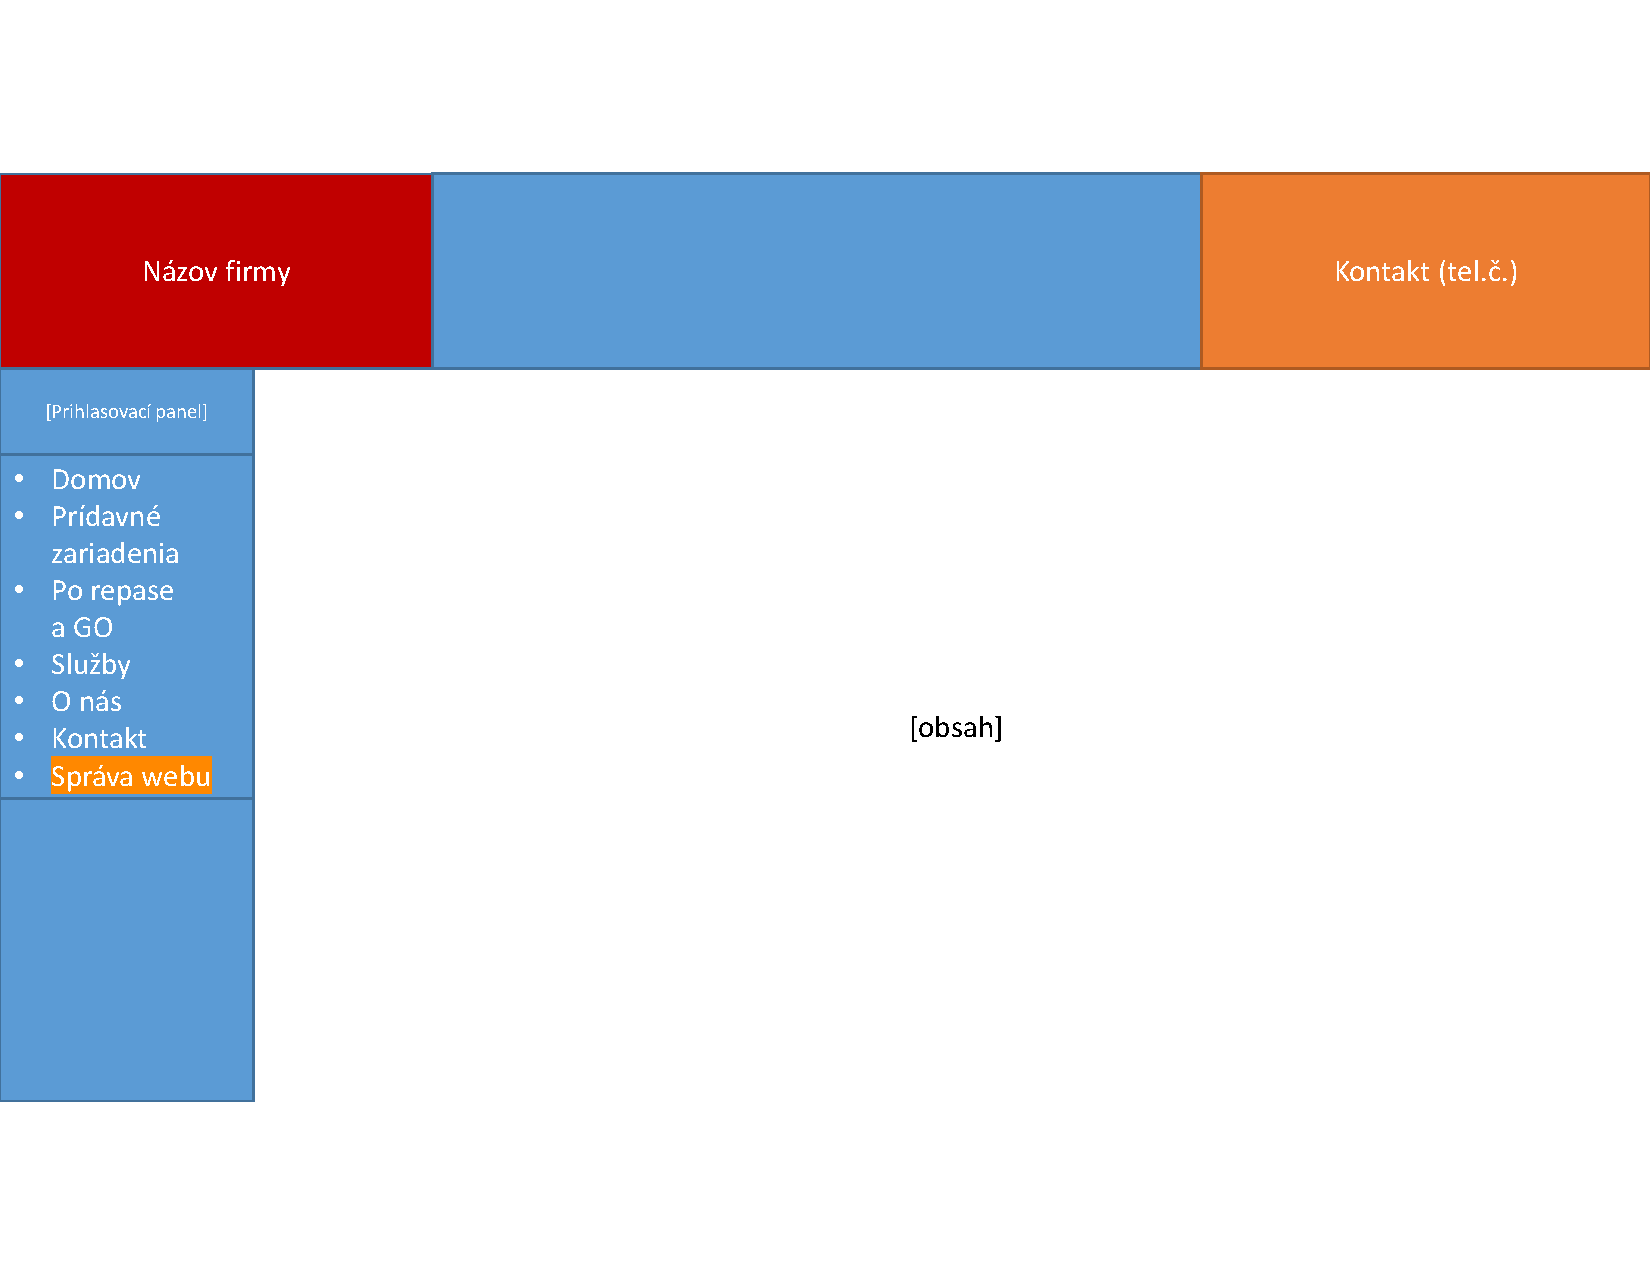
\includegraphics[width=140mm]{../img/UI concept/layout}
\caption{Návrh rozloženia aplikácie}
\label{layout}
\end{figure}

Všetky obrázky v~následujúcich podkapitolách (s~výnimkou grafov prechádzania medzi časťami aplikácie a~modálnym oknom) budú predstavovať obsahovú časť ak sa explicitne nepovie inak.

\section{Modálne okná}

V~následujúcich podkapitolách bude v~spojení s~mazaním položiek viackrát spomenuté modálne potvrdzovacie okno.

Okno má obsahovať vo~vrchnej časti nadpis a~v~centre text oznamujúci akciu. V~spodnej časti sa majú nachádzať tlačidlá~,,OK`` (pre~potvrdenie vymazania) a~,,Zrušiť`` (pre~zrušenie mazania).

Pre lepšiu predstavu viď obr.~\ref{confirmation modal}.

\begin{figure}[H]\centering
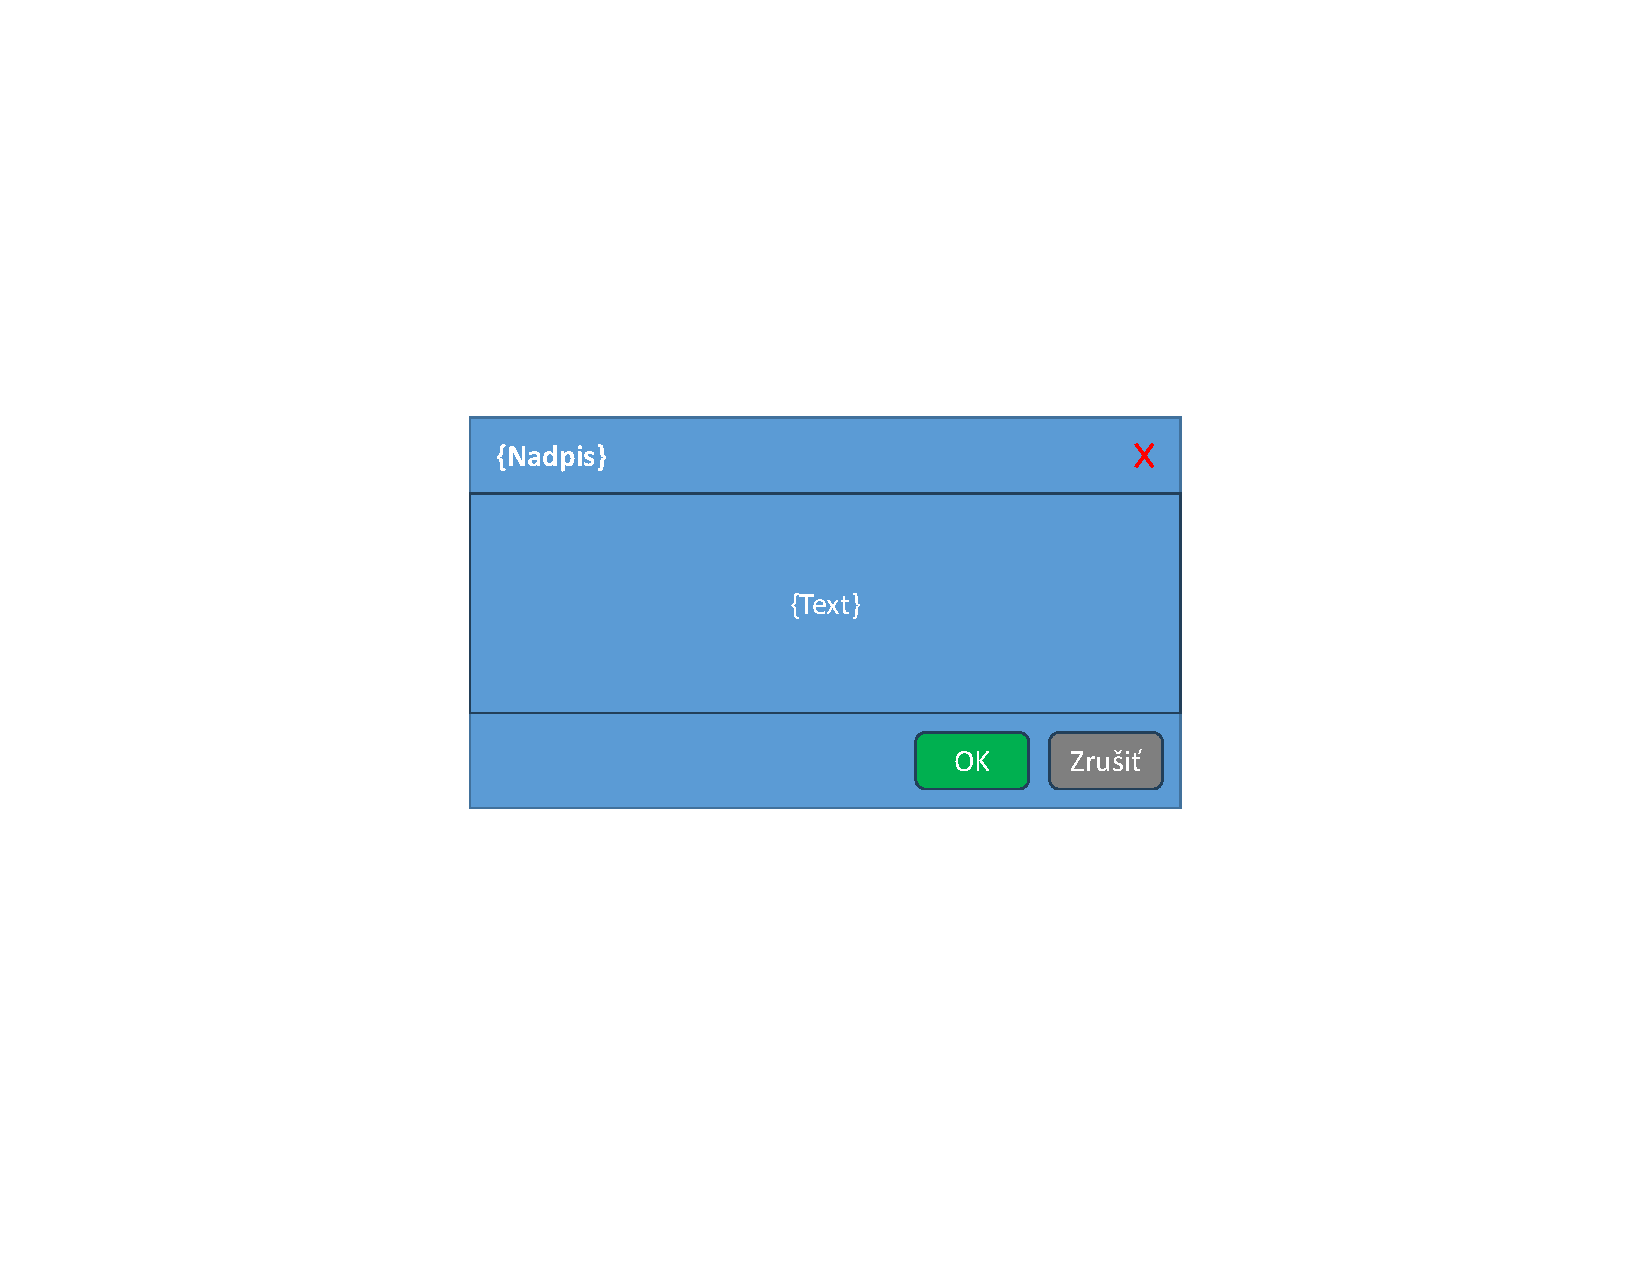
\includegraphics[width=140mm]{../img/UI concept/confirmation modal}
\caption{Potvrdzovacie modálne okno.}
\label{confirmation modal}
\end{figure}

\section{Splnenie P2 a P3}

V~tejto podkapitole si prejdeme časti aplikácie splňujúce požiadavky P2 a~P3, t.~j.~predstavenie hlavnej ponuky, bagrov, prídavných zariadení, a~takisto si z~časti ukážeme ako môže administrátor jednotlivé položky vytvárať, upravovať a~vymazovať (z~časti preto, lebo v~prípade bagrov bude existovať aj iný spôsob, o~ktorom si povieme neskôr).

Po~príchode na~stránku (alebo po~kliknutí na~odkaz ,,Domov`` v~navigácii) má byť užívateľovi zobrazená sekcia Domov s~vylistovanými kartami hlavnej ponuky. Administrátorovi sa na~každej z~kariet má zobrazovať tlačidlo, ktoré ho po~kliknutí presmeruje do~časti aplikácie, kde môže danú ponuku upravovať. Takisto sa v~sekcii Domov nachádza nad~kartami odkaz, ktorý má po~kliknutí administrátora presmerovať do~časti aplikácie, kde bude môcť vytvoriť novú hlavnú ponuku. Na~každej karte hlavnej ponuky má byť tlačidlo ,,Zobraziť``, ktoré má užívateľa presmerovať k~vylistovaným kartám (nových) bagrov. 

Kliknutím na~nejakú z~kariet bagrov má byť užívateľ presmerovaný do~časti aplikácie zobrazujúcej detail vybraného bagra~-- odtiaľ sa má byť (tentokrát už len) administrátor schopný dostať kliknutím na~tlačidlo ,,Upraviť`` do~časti aplikácie umožňujúcej upravovanie daného bagra.

Podobne má byť užívateľ schopný kliknúť na~odkaz ,,Prídavné zariadenia`` v~navigácii, ktorý ho presmeruje na~vylistované karty prídavných zariadení. Ak užívateľ klikne na~nejakú z~kariet, má byť presmerovaný na~detail vybraného prídavného zariadenia. Odtiaľ sa má byť (tentokrát už len) administrátor schopný dostať kliknutím na~tlačidlo ,,Upraviť`` do~časti aplikácie umožňujúcej upravovanie daného prídavného zariadenia.

Pre lepšie pochopenie prechádzania medzi jednotlivými časťami programu viď~obr.~\ref{p2 p3 graph}.

\begin{figure}[H]\centering
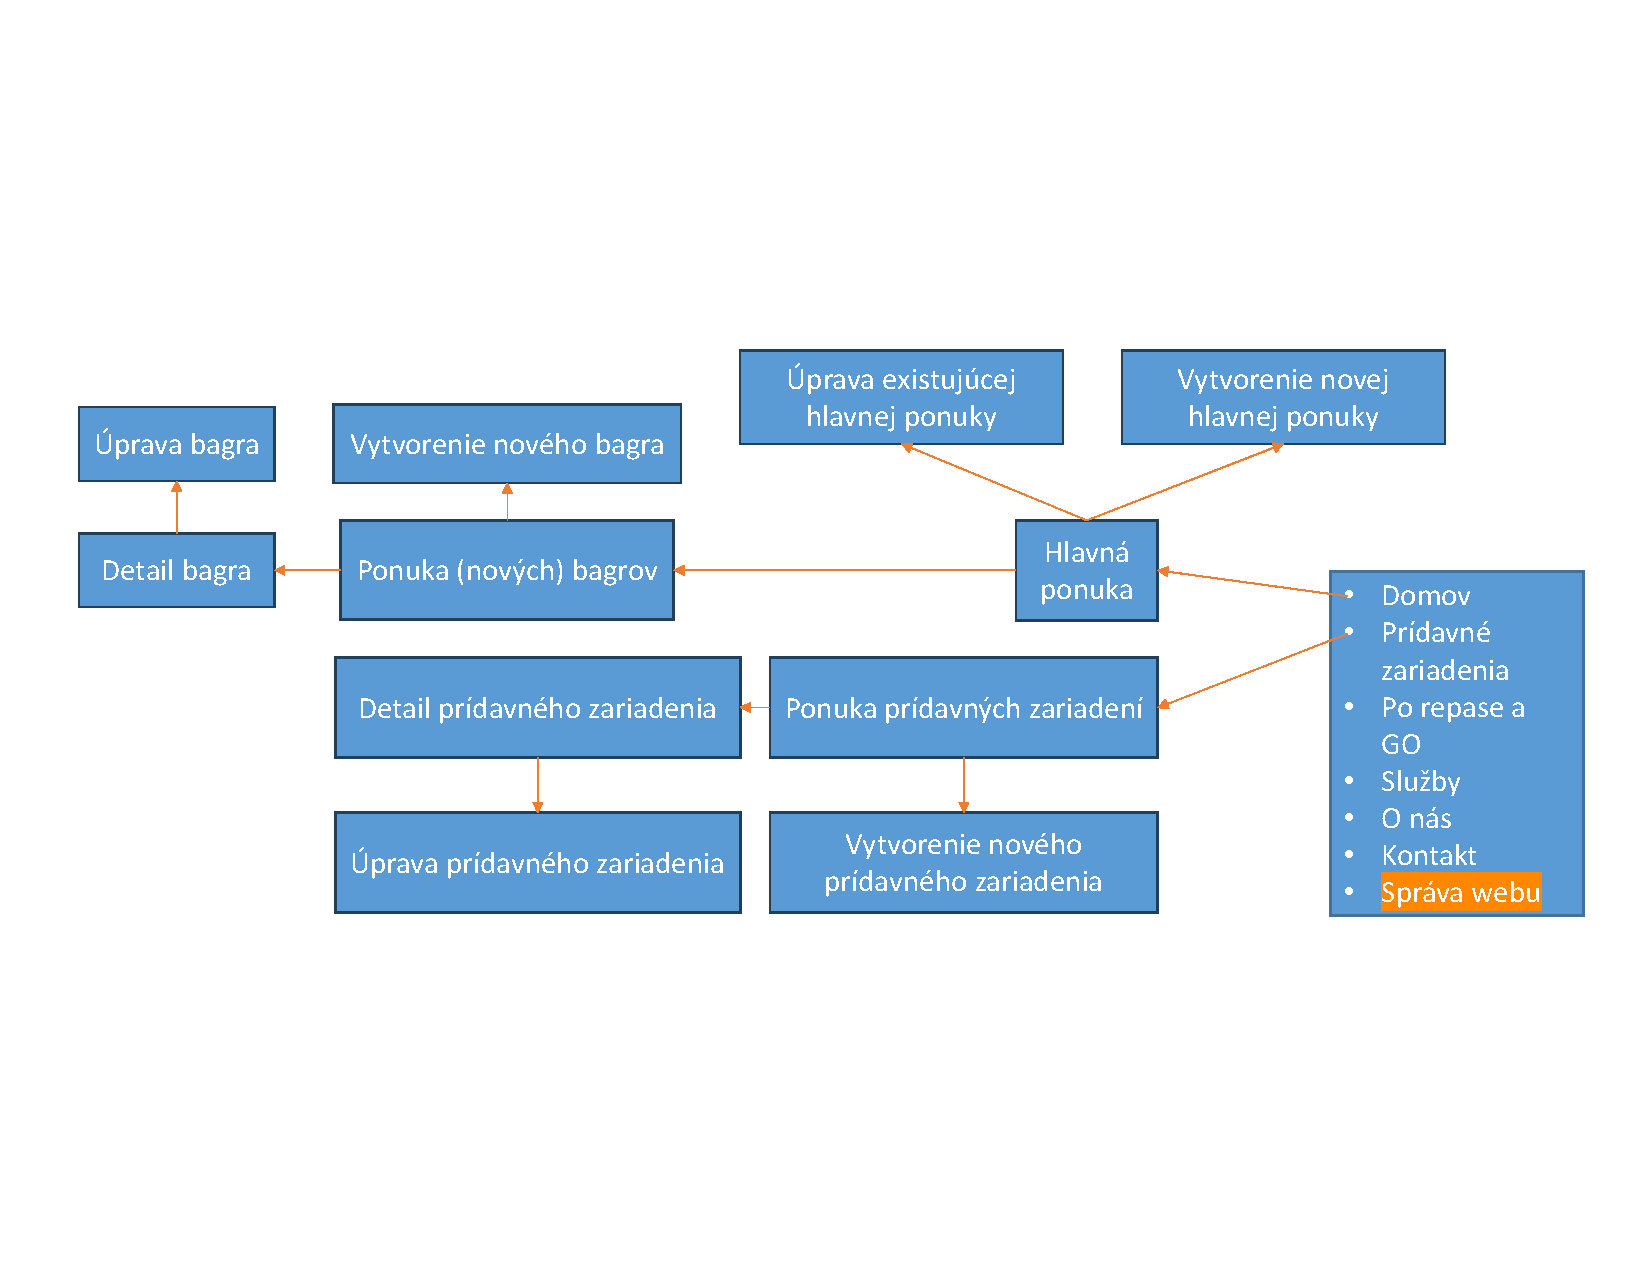
\includegraphics[width=140mm]{../img/UI concept/p2 p3 graph}
\caption{Prechádzanie medzi časťami aplikácie spĺňajúcimi požiadavky P2 a~P3.}
\label{p2 p3 graph}
\end{figure}

\subsection{Hlavná ponuka}

Po~príchode na~stránku sa užívateľ ocitne na~domovksej stránke, kde sú zobrazené karty hlavných ponúk (viď obr.~\ref{main offer cards}).

\begin{figure}[H]\centering
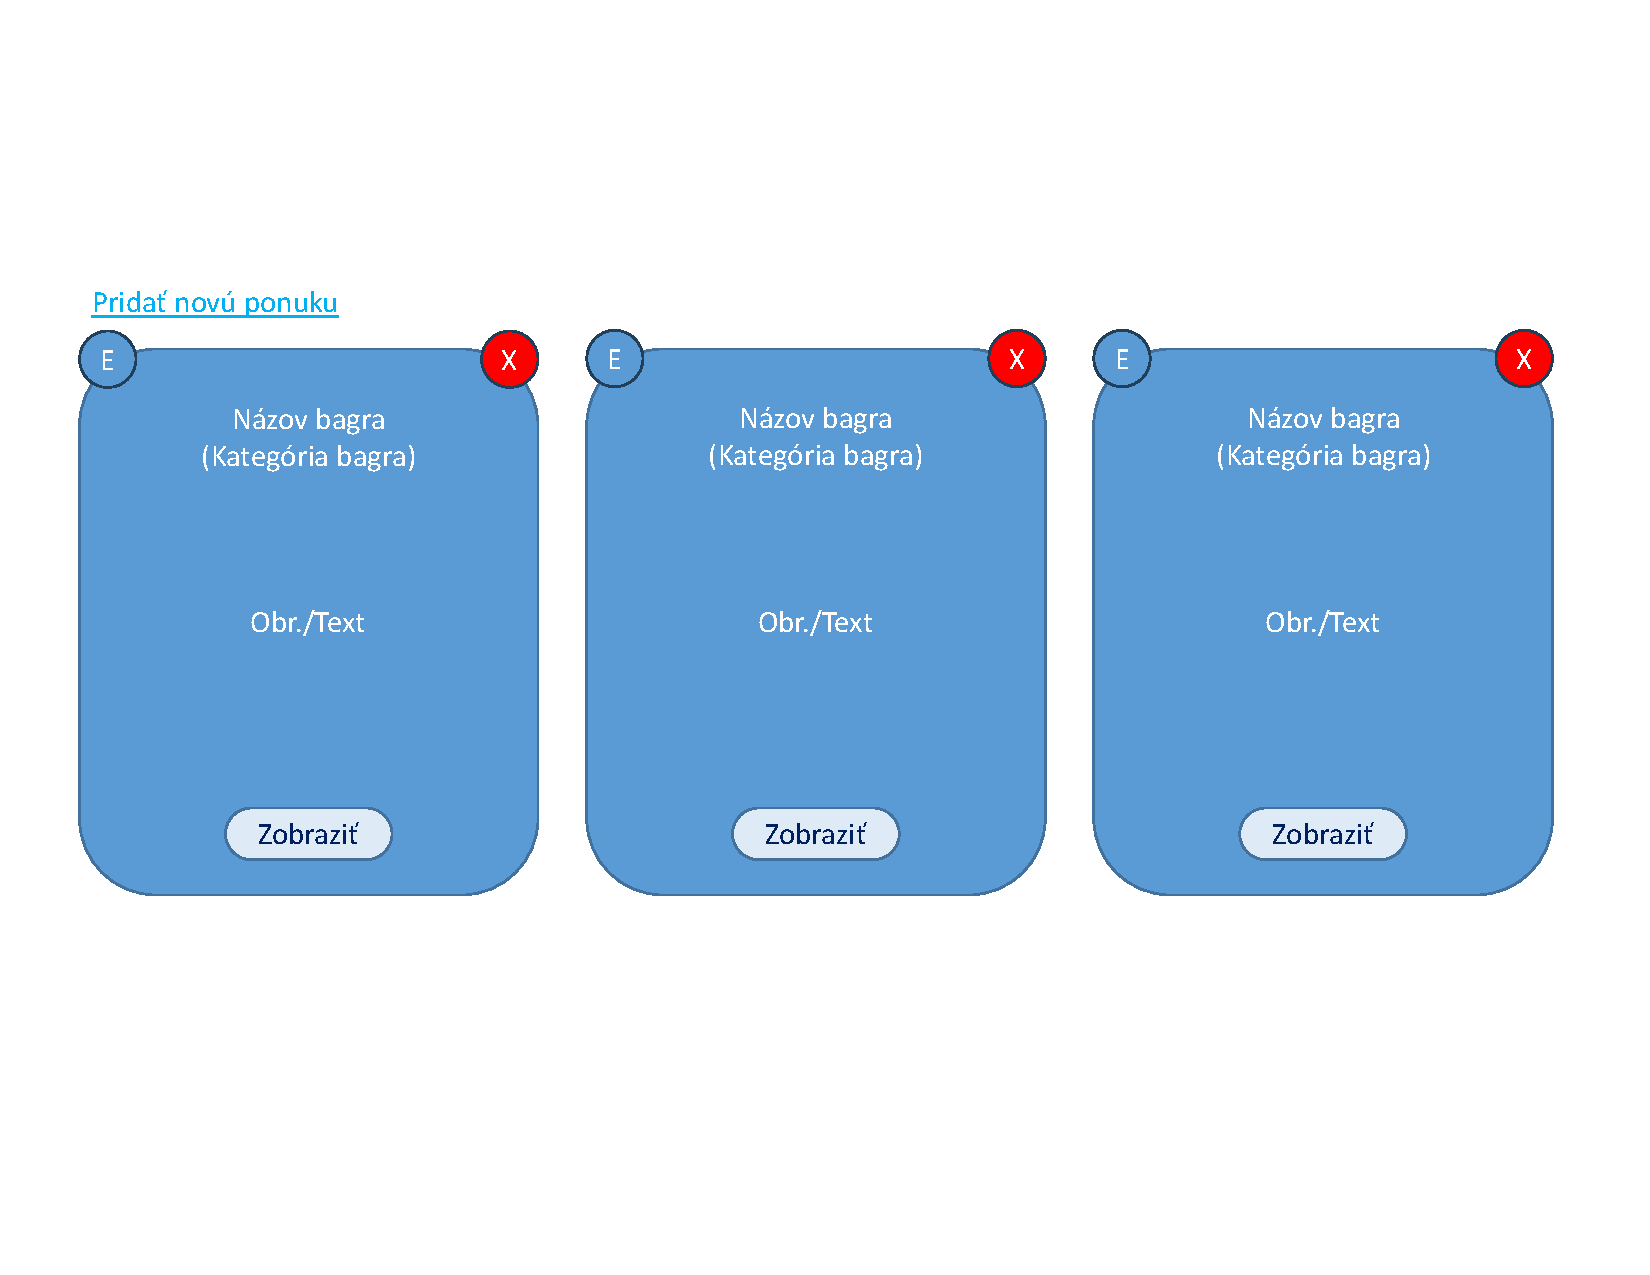
\includegraphics[width=140mm]{../img/UI concept/main offer cards}
\caption{Hlavná ponuka (úvodná stránka)}
\label{main offer cards}
\end{figure}

Každá z~kariet má zobrazovať fotku reprezentujúcu danú ponuku (resp.~typ bagra). Ak užívateľ prejde kurzorom na~kartu, tak sa má namiesto fotky zobraziť text opisujúci danú ponuku. 

Ďalej majú byť len pre~administrátorov zobrazené tlačidlá ,,E`` a~,,X`` vo~vrchných rohoch kariet, a~takisto nad~vylistovanými kartami odkaz ,,Pridať novú ponuku``.

Po~kliknutí na~tlačidlo ,,E`` nejakej z~hlavných ponúk má byť administrátor presmerovaný na~formulár vyplnený údajmi danej hlavnej ponuky, kde bude môcť túto ponuku upravovať.

Tlačidlo ,,X`` má slúžiť na~vymazanie danej hlavnej ponuky, po~kliknutí naň sa má zobraziť modálne potvrdzovacie okno s~nadpisom~,,Vymazať ponuku natrvalo`` a~textom ,,Naozaj chcete túto ponuku vymazať natrvalo?``.

Ďalej po~kliknutí na~odkaz ,,Pridať novú ponuku`` má byť administrátor presmerovaný na~prázdny formulár, kde bude môcť vytvoriť novú hlavnú ponuku.

Ďalej každá z~kariet má obsahovať tlačidlo~,,Zobraziť``, ktoré má po~kliknutí užívateľa presmerovať k~ponuke (nových) bagrov typu, ktorý prezentuje daná hlavná ponuka.

\subsection{Vytvorenie novej a úprava existujúcej hlavnej ponuky}

Ako bolo v~predošlej časti spomenuté, administrátor má byť schopný z~domovskej stránky (časť aplikácie kde majú byť vylistované hlavné ponuky) kliknutím na~odkaz ,,Pridať novú ponuku`` vytvoriť novú hlavnú ponuku a~kliknutím na~tlačidlo ,,E`` existujúcu hlavnú ponuku upravovať.

Či už v~prípade vytvárania novej, alebo~upravovania existujúcej hlavnej ponuky, má byť administrátor presmerovaný na~časť aplikácie s~formulárom umožňujúcim vložiť jednu fotku, vybrať z~možností typov bagrov, a~takisto napísať popis hlavnej ponuky. Všetky údaje až na popis sú povinné. Navyše po~vložení sa majú fotka a jej názov zobraziť vo~formulári.

Formulár má obsahovať tlačidlá ,,Uložiť`` (na~uloženie hlavnej ponuky) a~tlačidlo~,,Reset`` (na~vyprázdenie formulára).

Ak sú po~kliknutí na~tlačidlo~,,Uložiť`` povinné údaje nevyplnené, tak má na~to systém administrátora upozorniť prostrednictvom chybových správ pri~jednotlivých poliach.

Navyše nad~formulárom má byť v~prípade vytvárania novej hlavnej ponuky nadpis ,,Hlavné ponuky~-- vytvorenie nového záznamu`` a~v~prípade úpravy existujúcej hlavnej ponuky má byť nadpis ,,Hlavné ponuky~-- úprava existujúceho záznamu``.

Pre~lepšiu predstavu viď obr.~\ref{main offer form}.

\begin{figure}[H]\centering
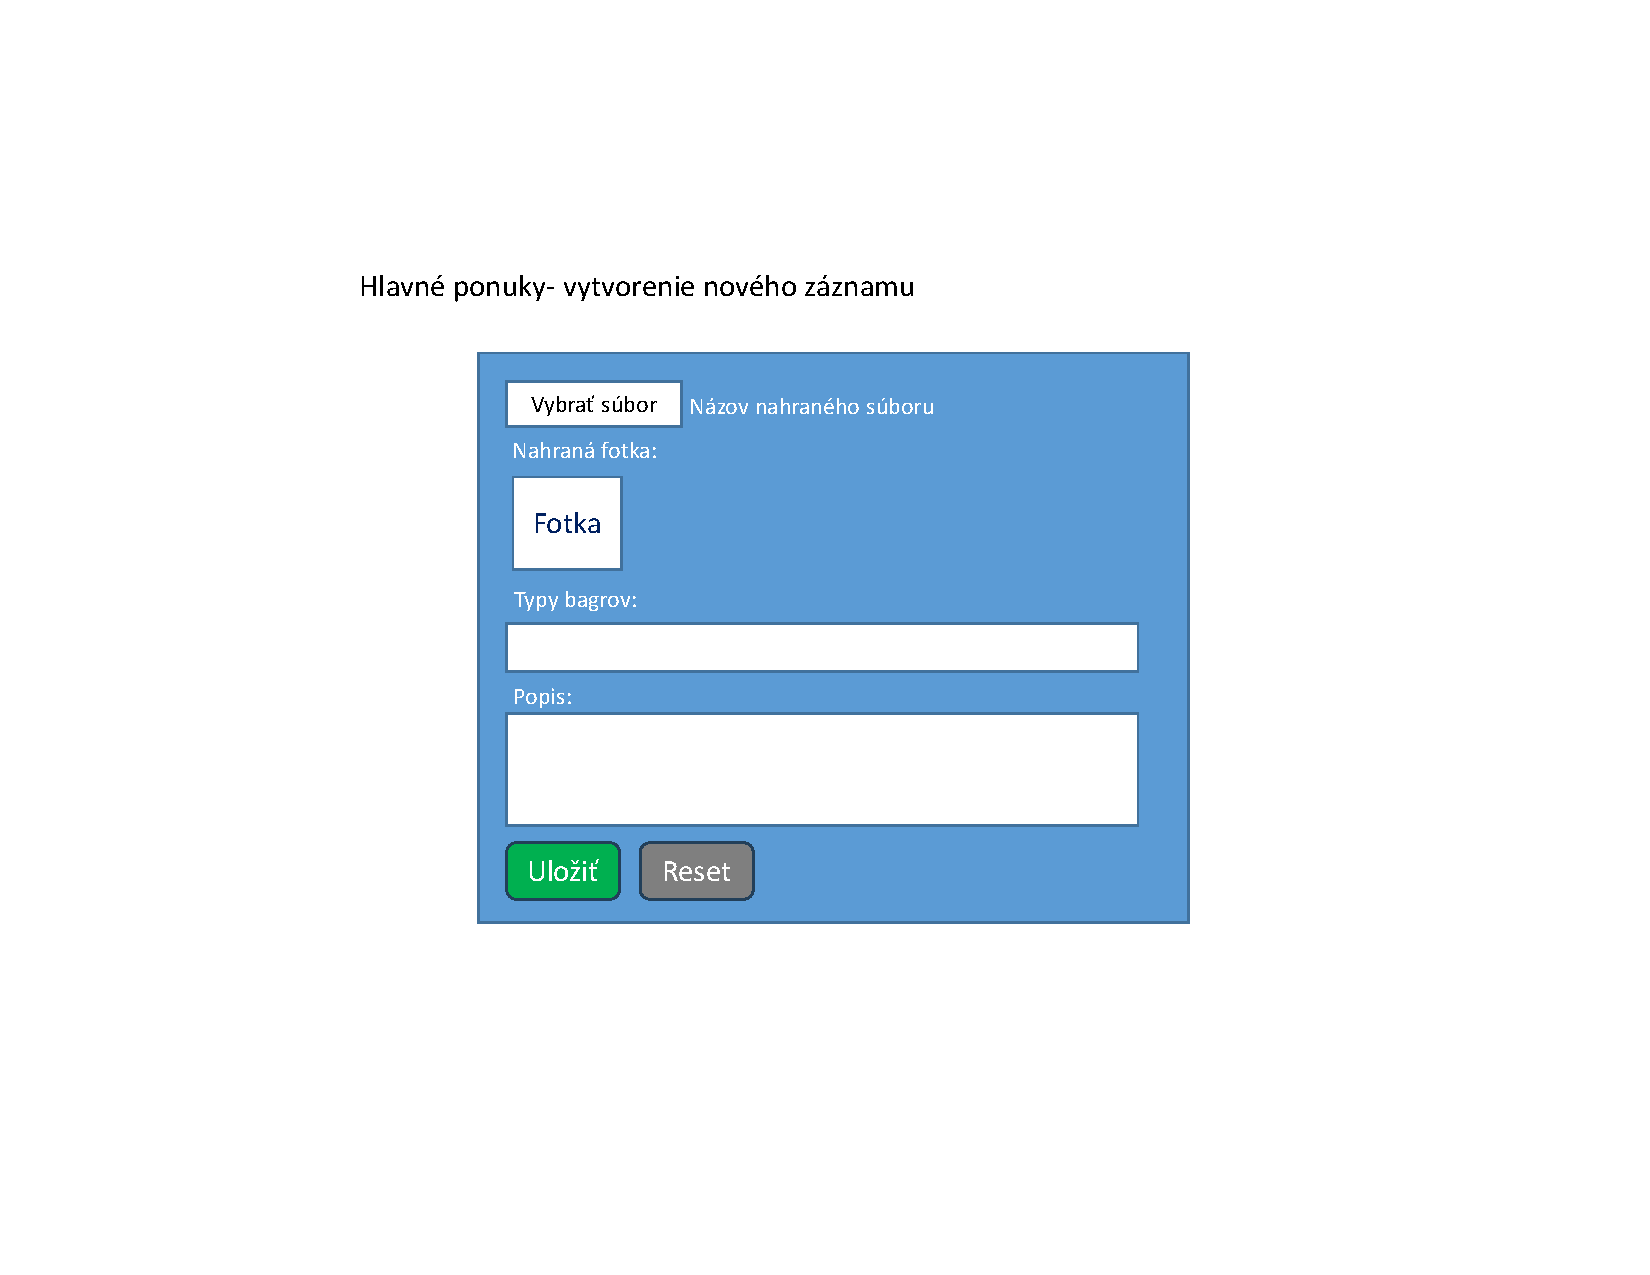
\includegraphics[width=140mm]{../img/UI concept/main offer form}
\caption{Časť aplikácie pre~vytvorenie hlavnej ponuky.}
\label{main offer form}
\end{figure}

\subsection{Ponuka (nových) bagrov}

Po~kliknutí na~tlačidlo ,,Zobraziť`` nejakej z~hlavných ponúk sa užívateľovi majú vylistovať karty strojov typu, ktorý prezentovala vybraná hlavná ponuka (viď obr.~\ref{excavator cards}). Medzi vylistovanými bagrami nemajú byť bagre určené iba pre~aukciu.

\begin{figure}[H]\centering
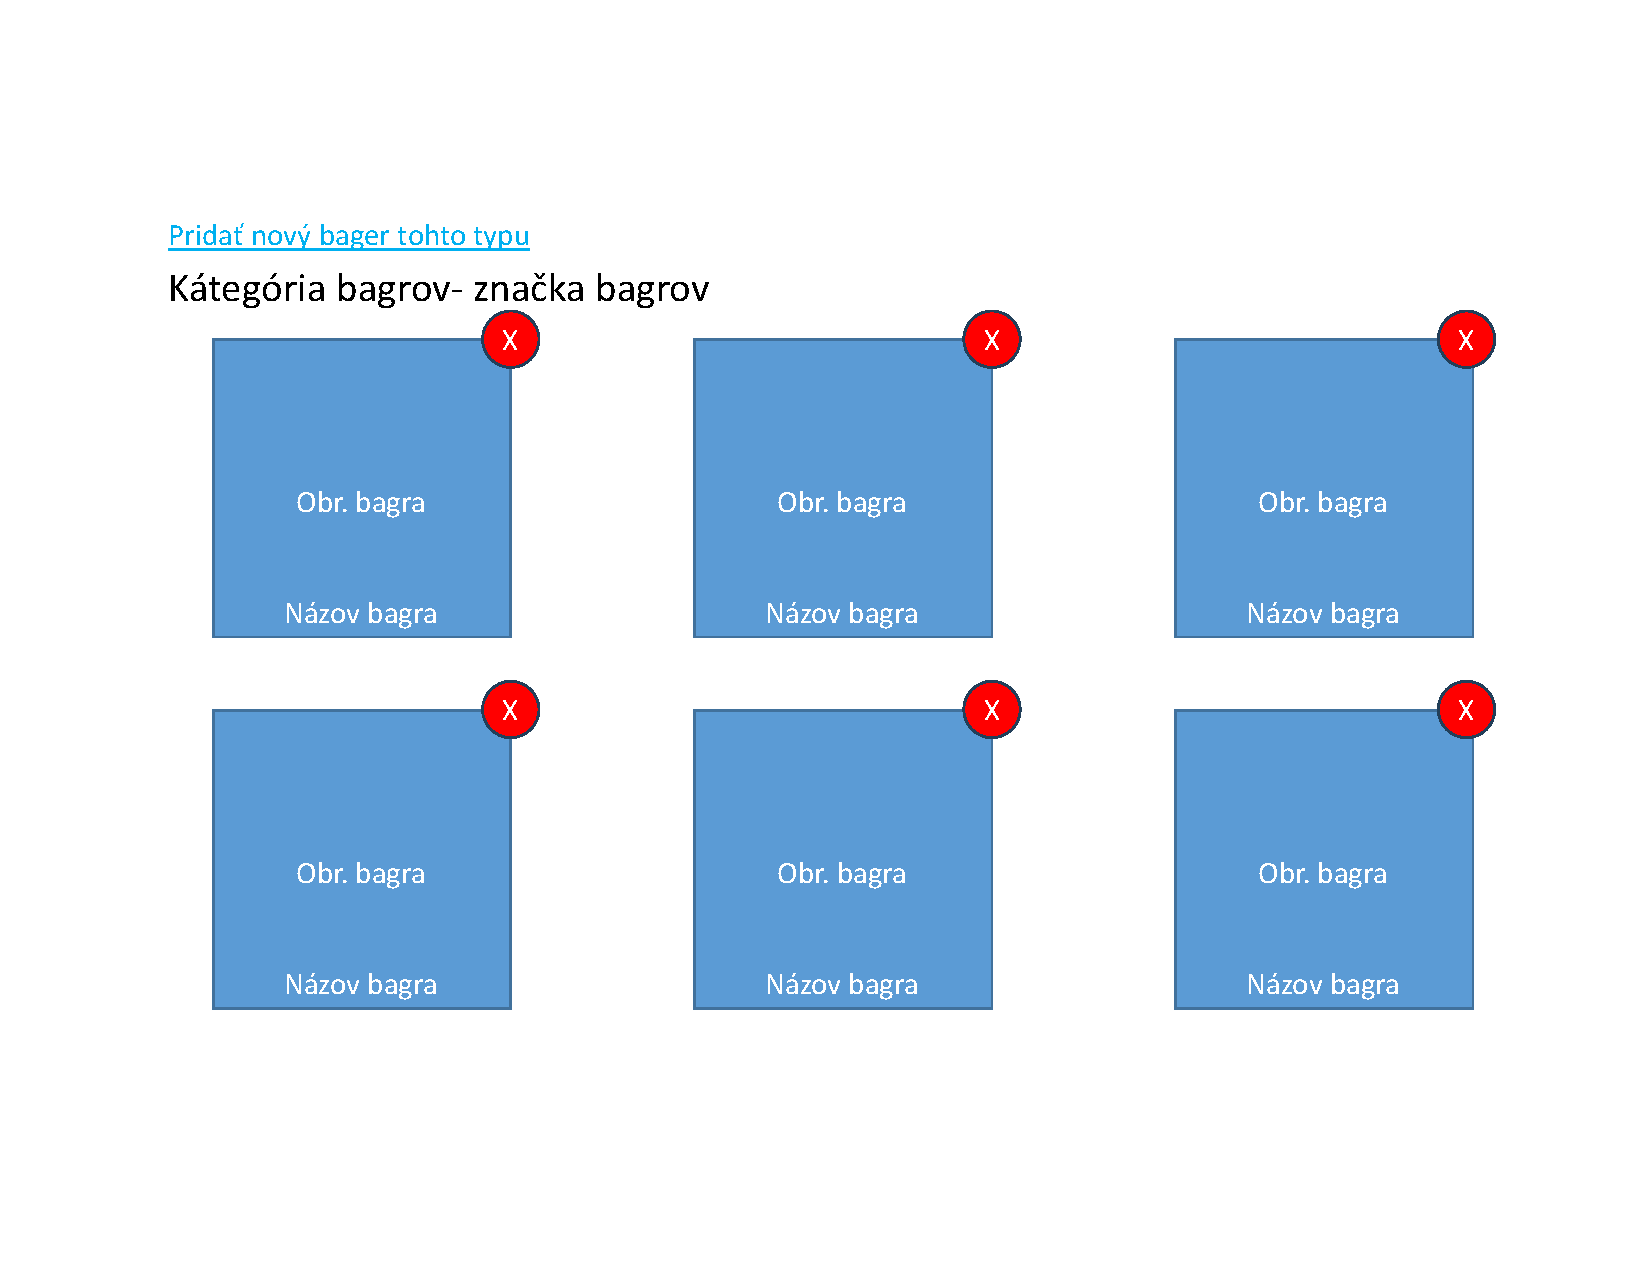
\includegraphics[width=140mm]{../img/UI concept/excavator cards}
\caption{Ponuka bagrov.}
\label{excavator cards}
\end{figure}

Nad~kartami bagrov sa má nachádzať nadpis v~tvare ,,\{Kategória vybraného typu bagrov\}~-- \{Značka vybraného typu bagrov\}`` (typ bagra určuje jeho kategóriu a~značku).

Okrem nadpisu sa má vo~vrchnej časti nachádzať aj odkaz~,,Pridať nový bager``, ktorý má užívateľa po~kliknutí presmeroať k~formuláru pre~vytvorenie nového stroja. Ak sa užívateľ dostal k~formuláru touto cestou, má mať vo~formulári predvyplnený typ stroja podľa typu vylistovaných strojov.

Každá z~kariet má mať v~pravom hornom rohu tlačidlo~,,X``, ktoré umožní daný stroj vymazať. Po~kliknutí naň sa má zobraziť modálne potvrdzovacie okno s~nadpisom~,,Vymazať bager natrvalo`` a~textom ,,Naozaj chcete tento bager vymazať natrvalo?``.

Tlačidlo~,,X`` aj odkaz~,,Pridať nový bager`` majú byť viditeľné iba pre~administrátorov.

Po~kliknutí na~nejakú z~kariet má byť užívateľ presmerovaný na~detail bagra.

\subsection{Ponuka prídavných zariadení}

Po kliknutí na~,,Prídavné zariadenia`` v~navigácii (viď~vľavo na~obr.~\ref{layout}) sa užívateľovi majú vylistovať karty prídavných zariadení (viď~obr.~\ref{additional equipment cards}).

\begin{figure}[H]\centering
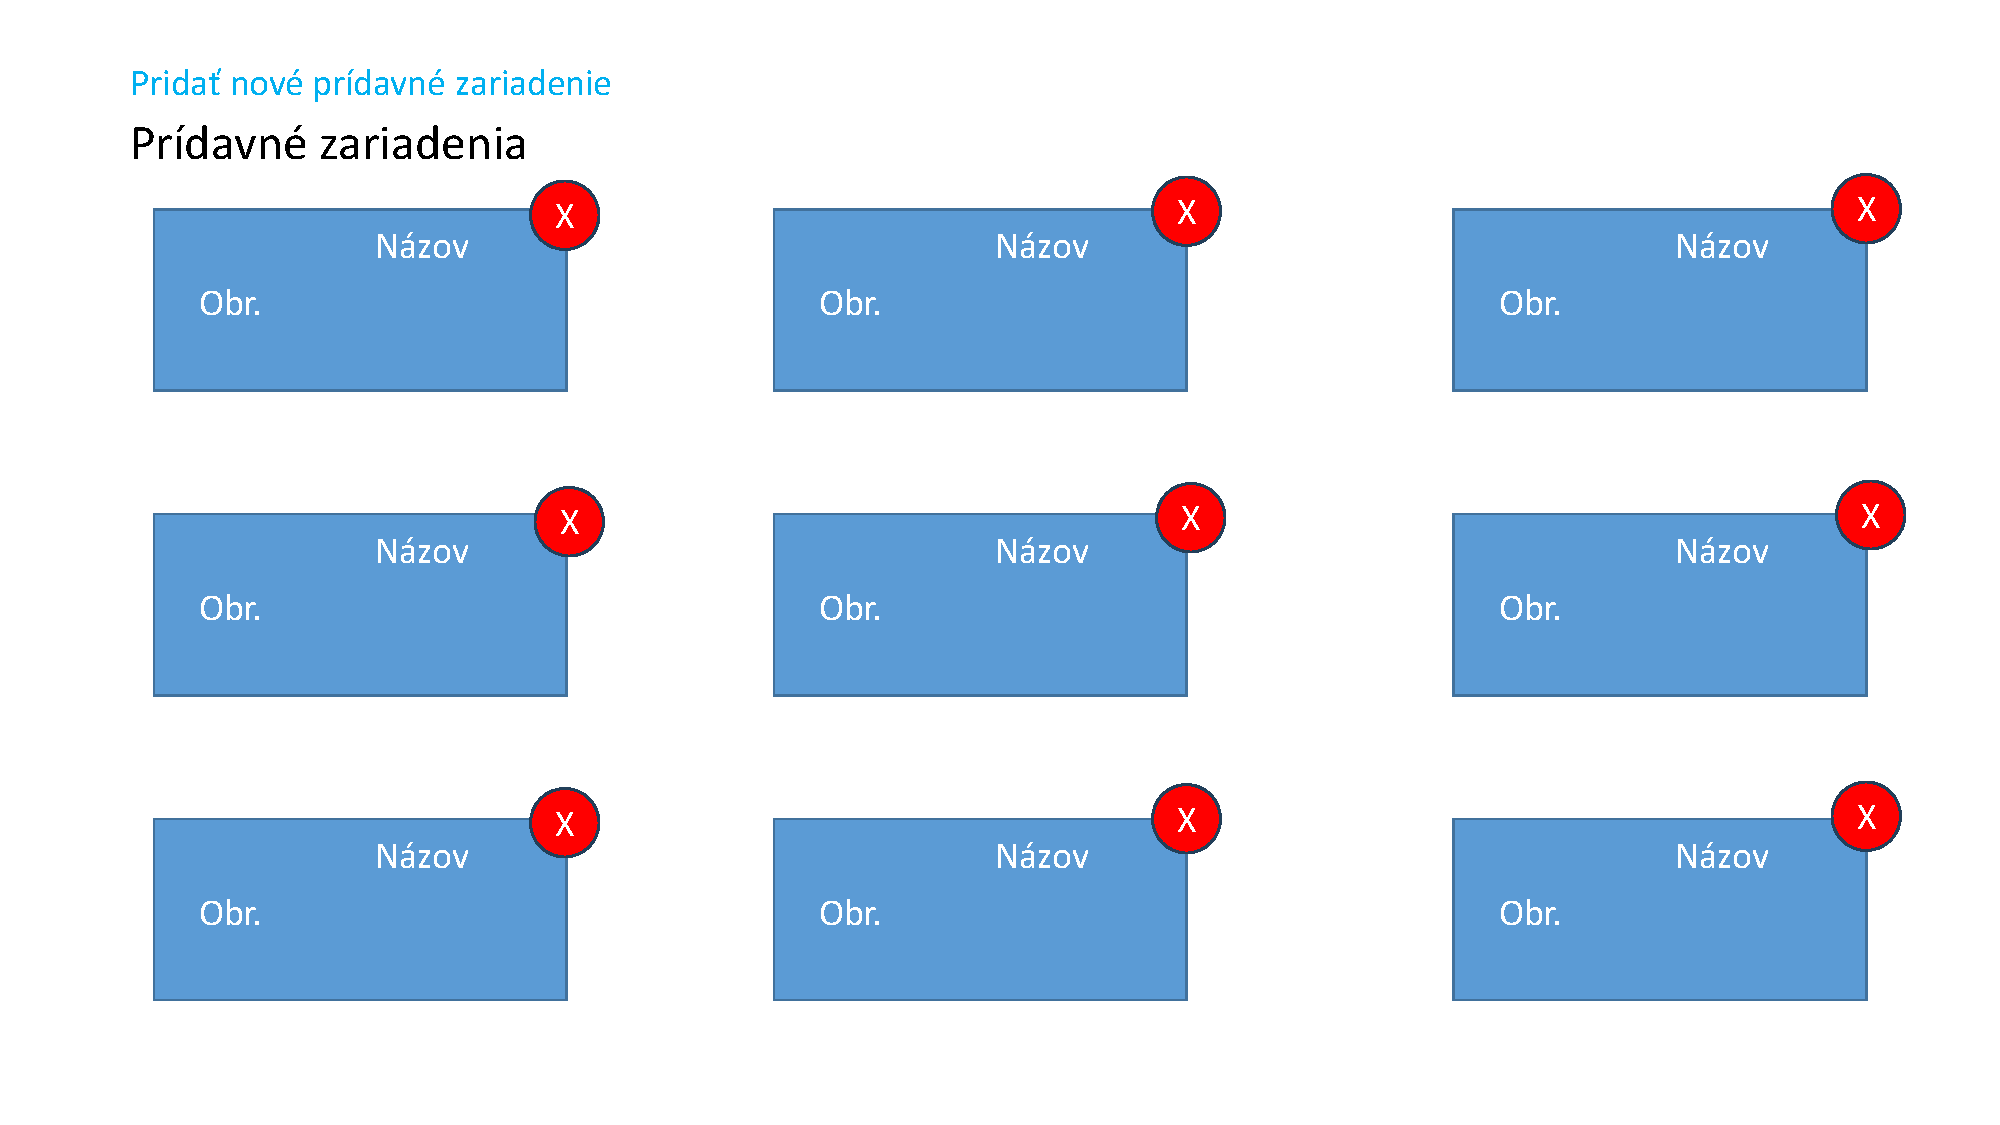
\includegraphics[width=140mm]{../img/UI concept/additional equipment cards}
\caption{Ponuka prídavných zariadení}
\label{additional equipment cards}
\end{figure}

Nad~kartami prídavných zariadení sa má nachádzať nadpis~,,Prídavné zariadenia``.

Okrem nadpisu sa má vo~vrchnej časti nachádzať aj odkaz~,,Pridať nové prídavné zariadenie``, viditeľný iba pre~administrátora, ktorý ho má  po~kliknutí presmerovať k~formuláru pre~vytvorenie nového prídavného zariadenia.

Každá z~kariet má mať v~pravom hornom rohu tlačidlo~,,X``, takisto viditeľné iba pre~administrátora, ktoré má umožniť dané prídavné zariadenie vymazať. Po~kliknutí na~tlačidlo~,,X`` sa má zobraziť modálne potvrdzovacie okno s~nadpisom~,,Vymazať prídavné zariadenie natrvalo`` a~textom ,,Naozaj chcete toto prídavné zariadenie vymazať natrvalo?``.

Po~kliknutí na~nejakú z~kariet má byť užívateľ presmerovaný na~detail prídavného zariadenia.

\subsection{Detail bagra, prídavného zariadenia}

Po~kliknutí na~nejakú z~kariet bagra alebo prídavného zariadenia sa má užívateľovi zobraziť stránka s~detailom vybraného predmetu (viď~obr.~\ref{detail}).

\begin{figure}[H]\centering
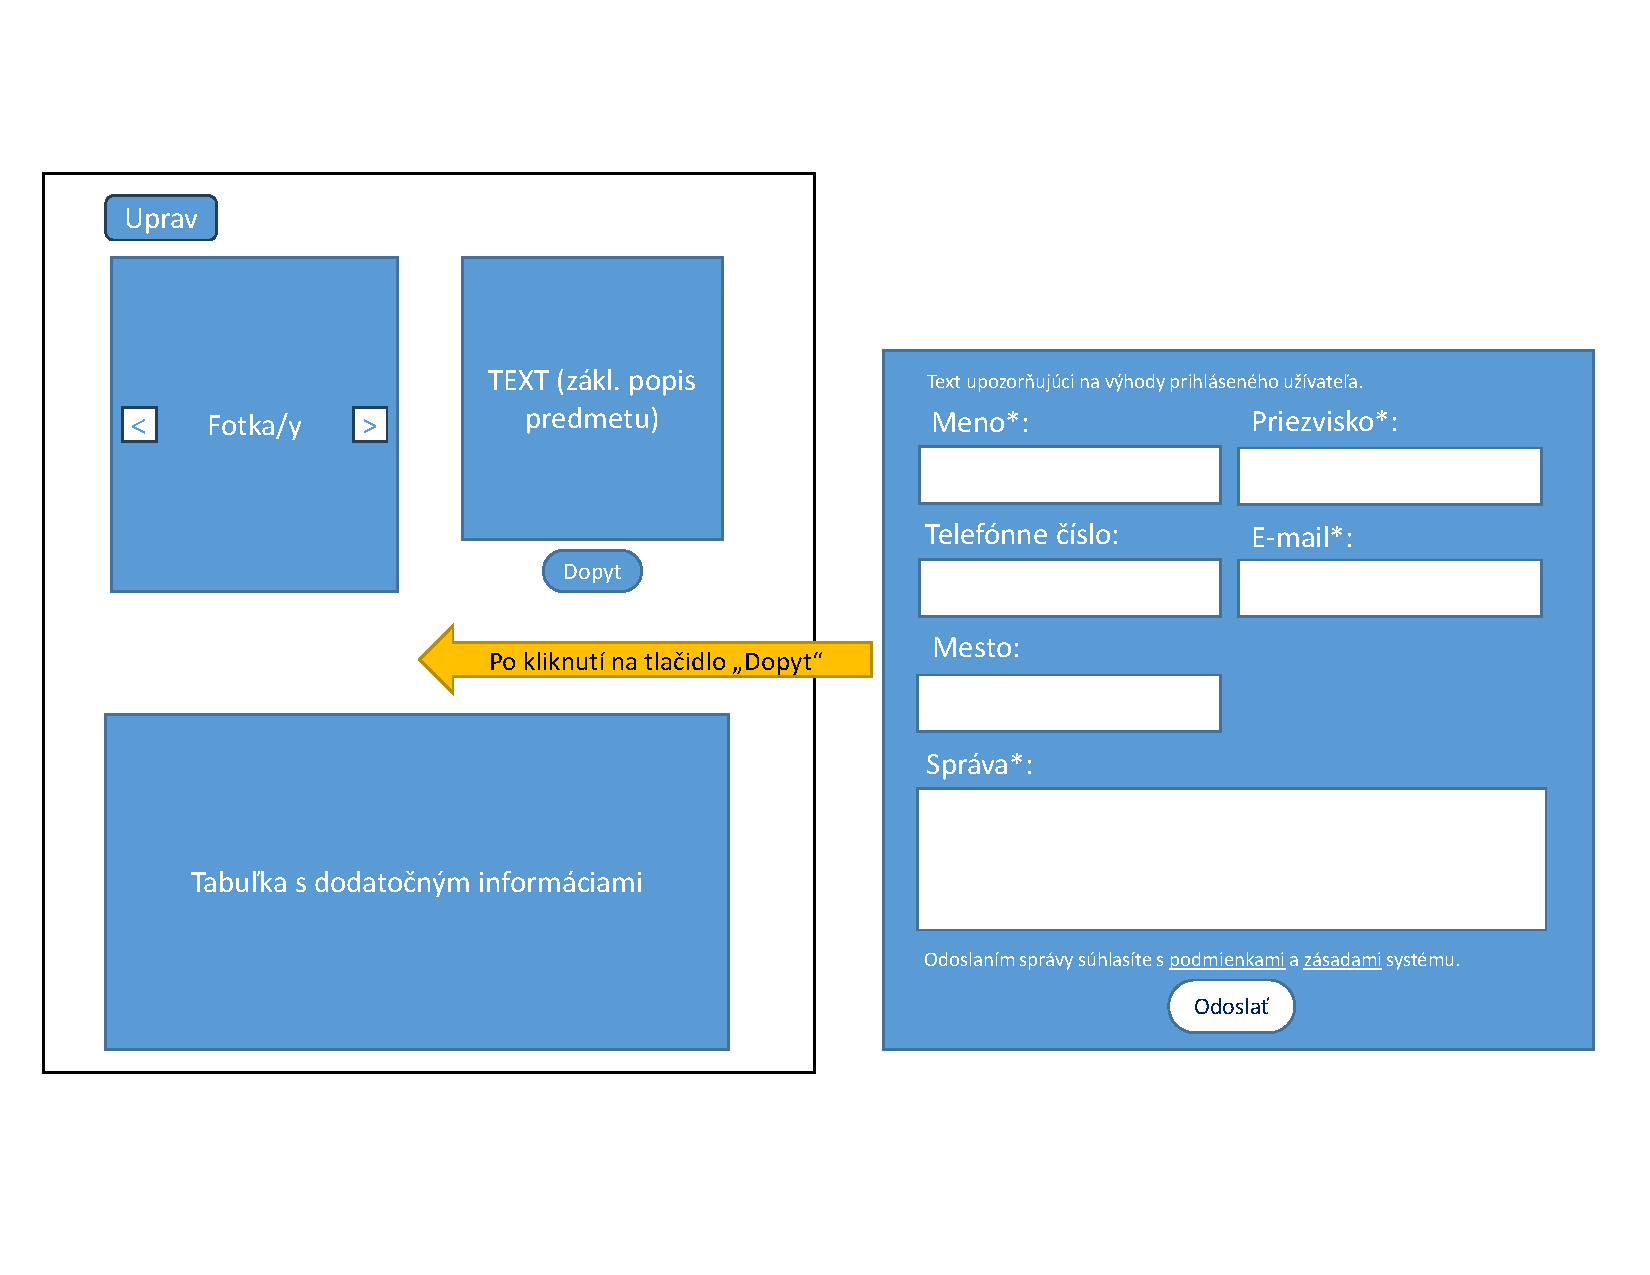
\includegraphics[width=140mm]{../img/UI concept/detail}
\caption{Detail bagra/prídavného zariadenia.}
\label{detail}
\end{figure}

V~tejto časti sa majú nachádzať fotky predmetu (klikaním na~tlačidlá šipiek vpravo, vľavo sa má prechádzať medzi fotkami predmetu). Ďalej sa má na~stránke nachádzať opis predmetu, a takisto tabuľka s~dodatočnými informáciami~-- v prípade bagra to majú byť jeho vlastnosti (napr. výška, šírka atď.), v~prípade pridavného zariadenia to majú byť údaje o~tom, akej značky, kategórie, a~taktiež pre~akú kategóriu bagrov je dané prídavné zariadenie.

Okrem toho sa má v~tejto časti ešte nachádzať tlačidlo~,,Dopyt``. Po~kliknutí naň sa má zobraziť formulár, ktorým bude môcť užívateľ odoslať dopyt na~daný predmet. Po~opätovnom kliknutí na~tlačidlo sa má formulár zatvoriť. Tlačidlo (a~ani formulár) sa nemajú zobrazovať administrátorom.

V~hornej časti sa má nachádzať tlačidlo~,,Upraviť``, ktoré má byť viditeľné iba pre~administrátorov. Po~kliknutí naň má byť administrátor presmerovaný na~formulár vybraného bagra (resp.~prídavného zariadenia). Pomocou formulára bude môcť administrátor daný bager (resp.~prídavné zariadenie) upravovať.

\subsection{Dopyt}
\label{dopyt}

V~predošlej časti textu bolo spomenuté, že v~detaile bagra alebo~prídavného zariadenia sa má nachádzať tlačidlo~,,Dopyt``, ktorým si bude môcť zákazník (nie administrátor) zobraziť (a~opätovným kliknutím schovať) formulár pre~odosielanie dopytu na~daný predmet.

Formulár má pre~neprihláseného zákazníka obsahovať povinné polia meno, priezvisko, email, správa, a~takisto nepovinné polia telefón, mesto. Pre~prihláseného zákazníka má formulár obsahovať iba povinné pole správa. Povinné polia majú byť označené hviezdičkou.

Okrem polí má v~sebe formulár obsahovať pre~neprihlásených zákazníkov správu upozorňujúcu na~to, že prihlásený užívateľ nemusí vypĺňať svoje osobné údaje. Takisto by mal formulár pre~neprihláseného užívateľa obsahovať upozornenie, že s~odoslaním správy súhlasí s~podmienkami a~zásadami aplikácie.

Ďalej má formulár obsahovať tlačidlo~,,Odoslať``, ktoré má zákazníkovi umožniť odoslanie dopytu.

Ak sú po~kliknutí na~tlačidlo~,,Odoslať`` povinné údaje nevyplnené, tak má na~to aplikácia užívateľa upozorniť chybovými správami pri~jednotlivých poliach.

Pre~lepšiu predstavu formulára viď~pravú časť obrázka~\ref{detail}.

\subsection{Vytvorenie nového a úprava existujúceho bagra}

Kliknutím na~odkaz~,,Pridať nový bager``, ktorý sa má nachádzať v~časti s~vylistovanými (novými) bagrami, má byť administrátor presmerovaný do~časti aplikácie, kde bude môcť vytvoriť nový bager.

Podobne kliknutím na~tlačidlo~,,Upraviť``, ktoré sa má nachádzať v~časti s~detailom bagra, má byť administrátor presmerovaný do~časti aplikácie, kde bude môcť existujúci bager upravovať.

Obe časti majú obsahovať formulár umožňujúci vloženie viacerých fotiek, názvu bagra, zadanie jeho popisu, uvedenie či je stroj určený iba pre~aukciu, tiež bude môcť administrátor vybrať, ktoré náhradné diely patria do~daného bagra, a~takisto vybrať z~možností typov bagrov. Podľa vybraného typu bagra sa majú zobraziť vlastnosti ním určené a~administrátor bude môcť vyplniť ich hodnoty. Fotky, názov bagra a jeho typ sú povinné údaje.

Navyše po~vložení sa majú fotky a~ich počet zobraziť vo formulári. V~pravom hornom rohu každej zobrazenej fotky sa má nachádzať tlačidlo~,,X``, ktorým môže administrátor fotku odstrániť.

Formulár taktiež obsahuje tlačidlá ,,Uložiť`` (na~uloženie bagra) a~,,Reset`` (na~vyprázdenie formulára).

Ak sú po~kliknutí na~tlačidlo~,,Uložiť`` povinné údaje nevyplnené, tak má na~to systém administrátora upozorniť prostrednictvom chybových správ pri~jednotlivých poliach.

Navyše nad~formulárom má byť v~prípade vytvárania nového bagra nadpis ,,Bagre~-- vytvorenie nového záznamu`` a~v~prípade úpravy existujúceho bagra má byť nadpis ,,Bagre~-- úprava existujúceho záznamu``.

Pre~lepšiu predstavu viď~obr.~\ref{excavator form}.

\begin{figure}[H]\centering
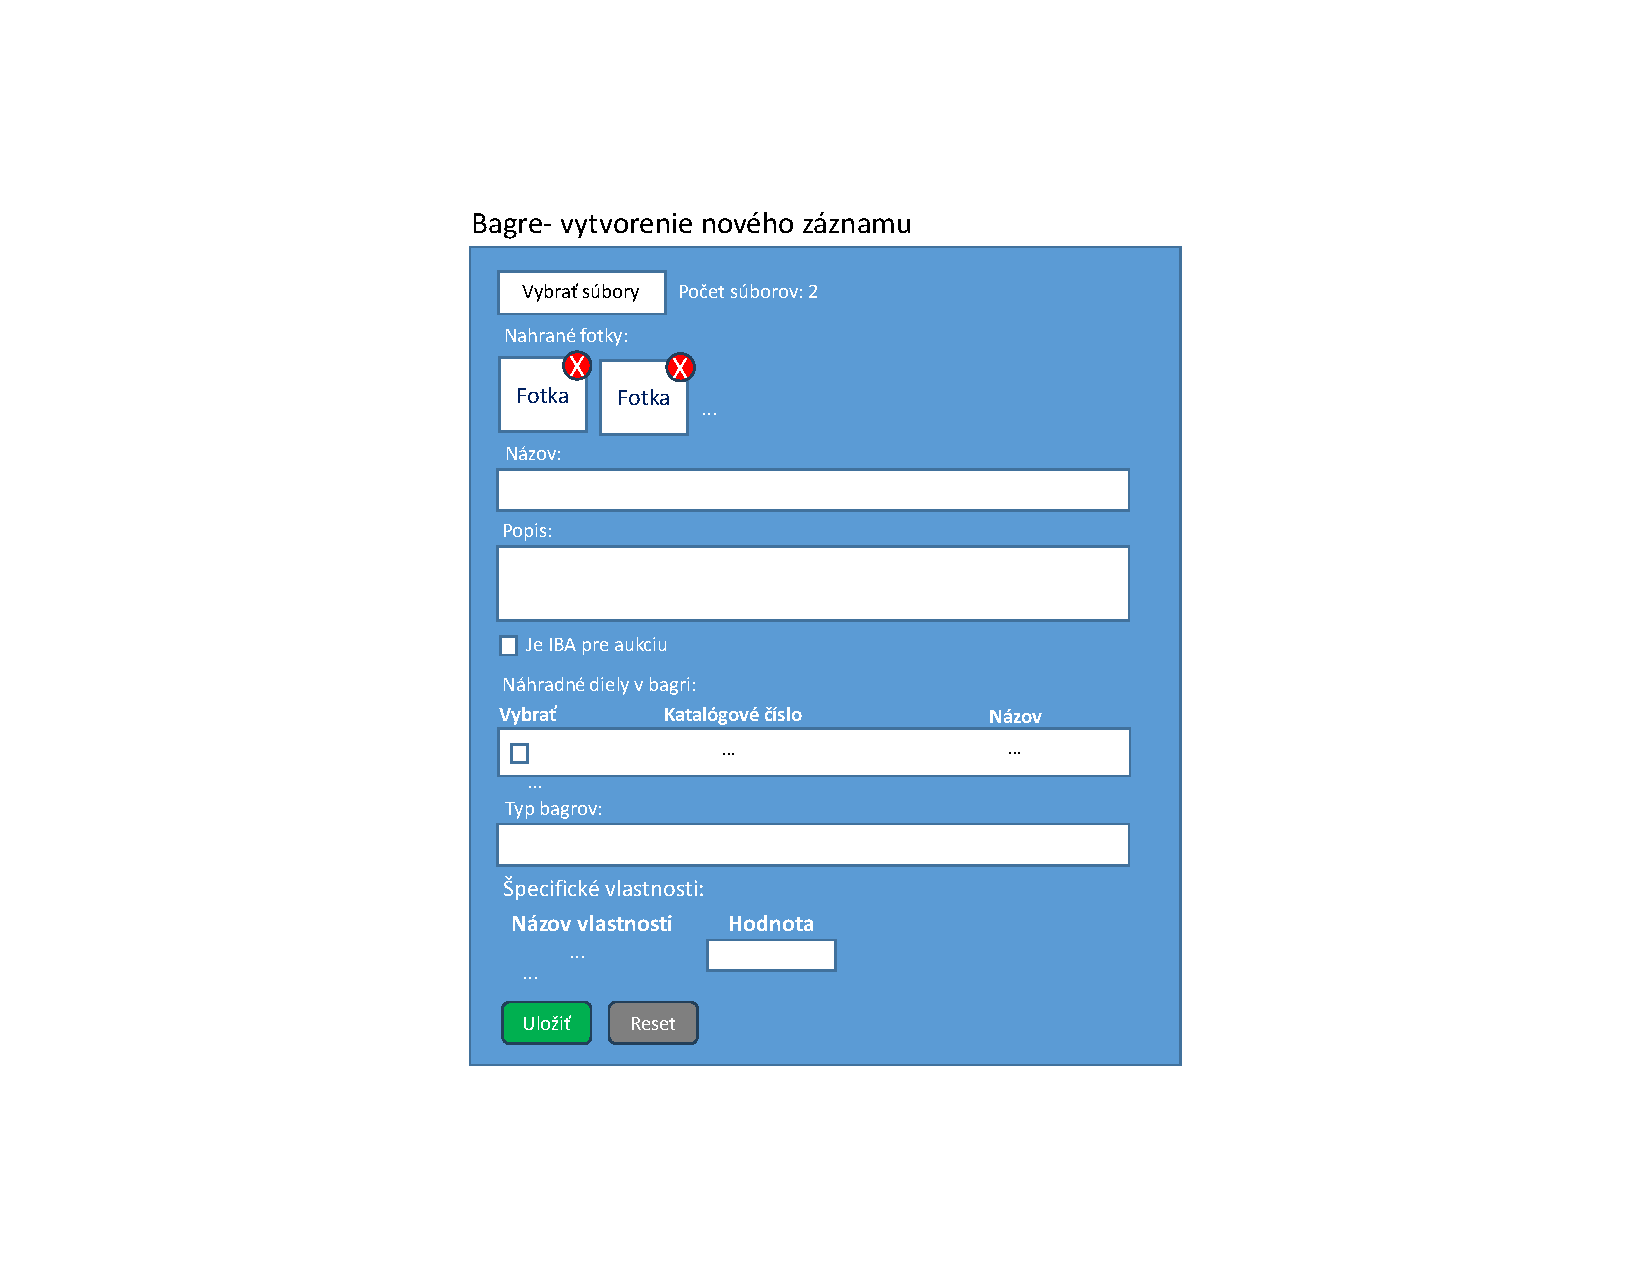
\includegraphics[width=140mm]{../img/UI concept/excavator form}
\caption{Časť aplikácie pre~vytvorenie bagra.}
\label{excavator form}
\end{figure}

\subsection{Úprava bagrov, ktoré nie sú v ponuke (nových) bagrov}

V~predošlom texte bolo napísané, že administrátor sa bude môcť cez~karty hlavných ponúk dostať k~ponuke (nových) bagrov a~cez nich k~detailu bagra, kde môže kliknutím na~tlačidlo ,,Upraviť`` upravovať daný bager. Ale ak by administrátor vytvoril bager typu, pre~ktorý neexistuje hlavná ponuka alebo~bager určený iba pre~aukciu, tak by sa bager nezobrazoval medzi ponukou (nových) bagrov.

Preto bude pre~takéto bagre (a~tiež pre~položky s~podobným problémom) vyhradená osobitná časť aplikácie, kde ich bude môcť administrátor spravovať (t.~j.~vytvárať, upravovať a mazať). Viac o~tejto časti aplikácie v~podkapitole~\ref{splnenie p5 p7 a sprava predmetov}.

\subsection{Vytvorenie nového a úprava existujúceho prídavného zariadenia}

Kliknutím na~odkaz~,,Pridať nové prídavné zariadenie``, ktorý sa má nachádzať v časti s~vylistovanými prídavnými zariadeniami, má byť administrátor presmerovaný do~časti aplikácie, kde bude môcť vytvoriť nové prídavné zariadenie.

Podobne kliknutím na~tlačidlo~,,Upraviť``, ktoré sa má nachádzať v~časti s~detailom prídavného zariadenia, má byť administrátor presmerovaný do~časti aplikácie, kde bude môcť existujúce prídavné zariadenie upravovať.

Obe časti majú obsahovať formulár umožňujúci vloženie viacerých fotiek, vybranie kategórie bagrov (pre~ktoré je prídavné zariadenie určené), vybranie jeho kategórie, vybranie značky, a~takisto zadanie názvu a~popisu prídavného zariadenia. Okrem popisu sú všetky údaje povinné.

Navyše po~vložení sa majú fotky a~ich počet zobraziť vo~formulári. V~pravom hornom rohu každej zobrazenej fotky sa má nachádzať tlačidlo~,,X``, ktorým môže administrátor fotku odstrániť.

Formulár taktiež obsahuje tlačidlá ,,Uložiť`` (na~uloženie prídavného zariadenia) a~,,Reset`` (na~vyprázdenie formulára).

Ak sú po~kliknutí na~tlačidlo~,,Uložiť`` povinné údaje nevyplnené, tak má na~to systém administrátora upozorniť prostrednictvom chybových správ pri~jednotlivých poliach.

Navyše nad~formulárom má byť v~prípade vytvárania nového bagra nadpis ,,Prídavné zariadenia~-- vytvorenie nového záznamu`` a~v~prípade úpravy existujúceho prídavného zariadenia má byť nadpis ,,Prídavné zariadenia~-- úprava existujúceho záznamu``.

Pre~lepšiu predstavu viď~obr.~\ref{additional equipment form}.

\begin{figure}[H]\centering
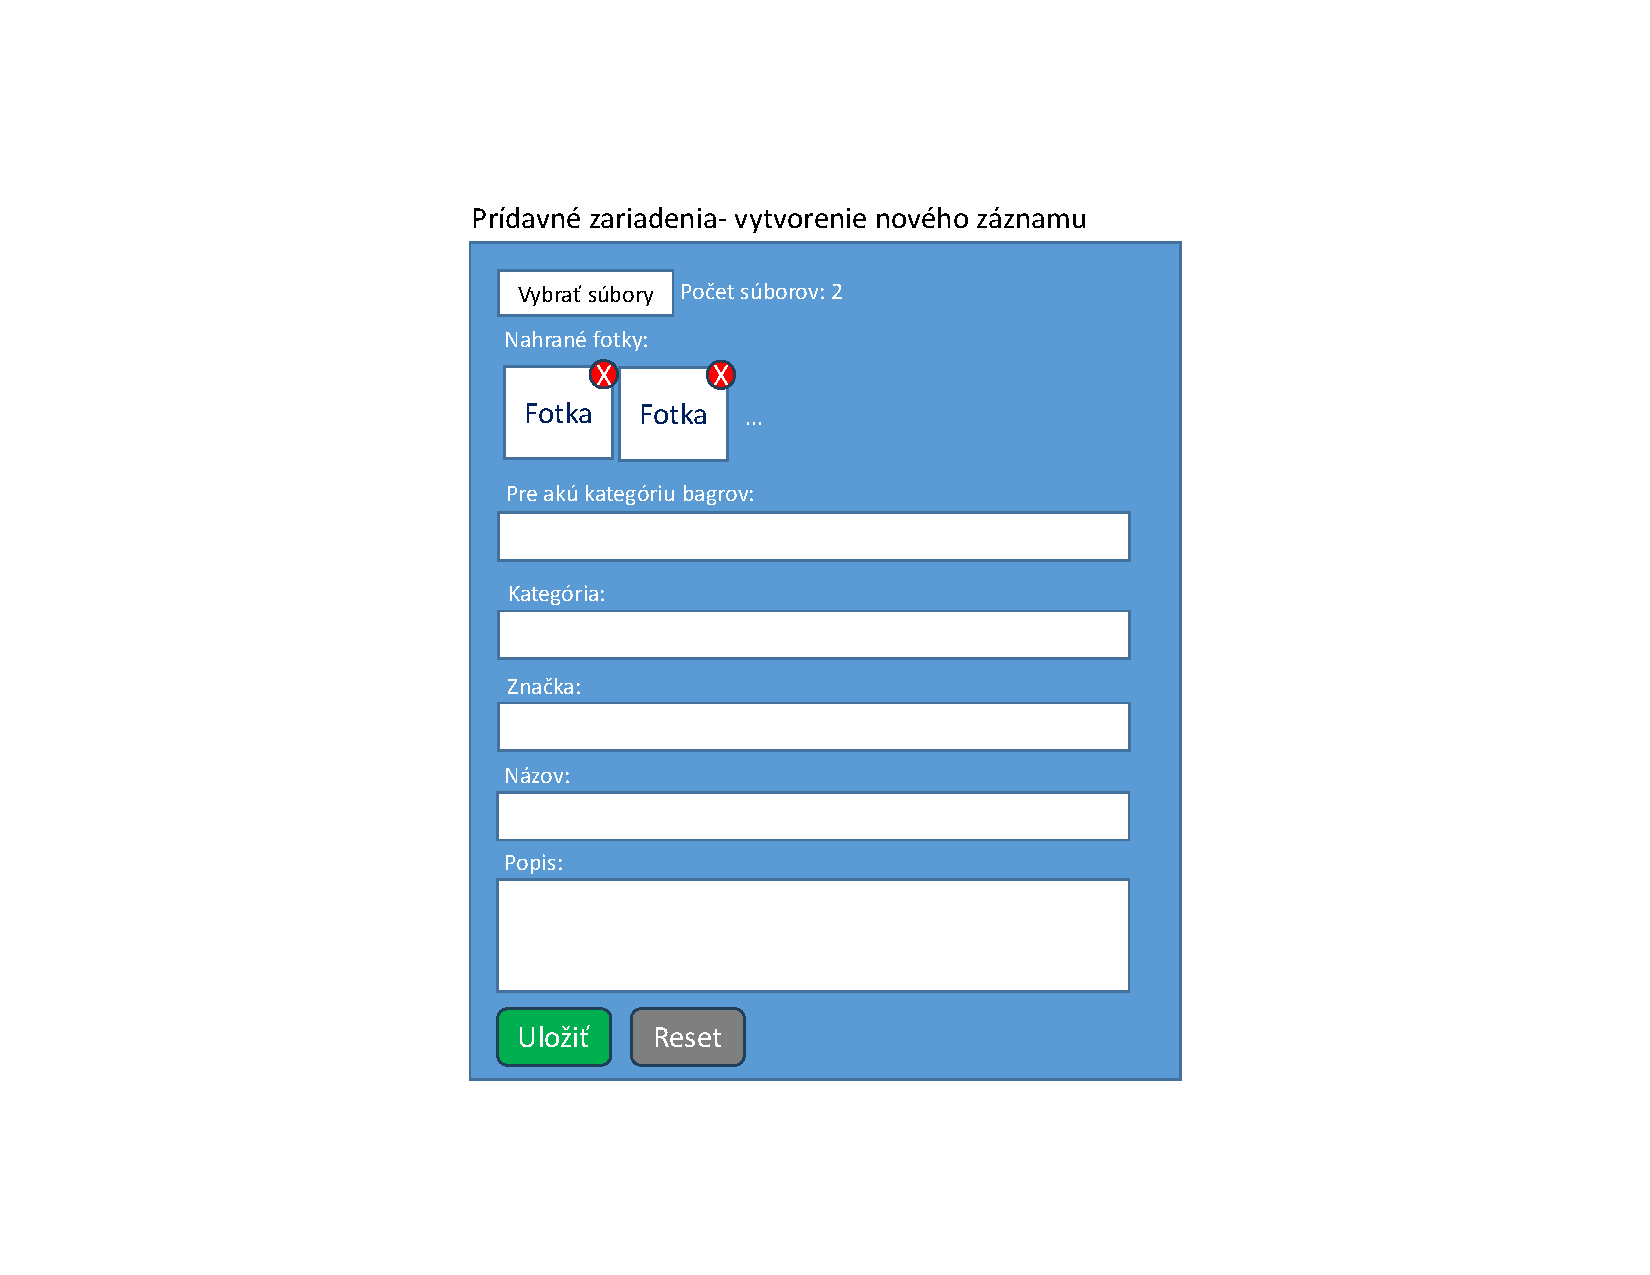
\includegraphics[width=140mm]{../img/UI concept/additional equipment form}
\caption{Časť aplikácie pre~vytvorenie prídavného zariadenia.}
\label{additional equipment form}
\end{figure}

\section{Splnenie P4}

V~tejto podkapitole si prejdeme časti aplikácie splňujúce požiadavku P4, t.~j.~predstavenie aukčnej ponuky, časti umožňujúce administrátorovi vytvárať (a~upravovať) aukčné ponuky, a~takisto časti umožňujúce zákazníkom ponúkať sumy do~dražby.

Po~kliknutí na~odkaz~,,Po repase a GO`` v~navigácii má byť užívateľovi zobrazená časť aplikácie s~vylistovanými kartami aukčnej ponuky. Nad~kartami (tentokrát už iba) administrátorovi sa má zobrazovať odkaz~,,Pridať novú aukčnú ponuku``, ktorým sa bude môcť dostať do~časti aplikácie s~prázdnym formulárom pre~vytvorenie novej aukčnej ponuky.

Po~kliknutí na~nejakú z~kariet sa má užívateľovi zobraziť detail aukčnej ponuky. V~časti detailu sa má iba administrátorovi zobrazovať tlačidlo~,,Upraviť``, ktorým sa bude môcť dostať do~časti aplikácie, kde môže danú ponuku upravovať a~iba zákazníkovi tlačidlo~,,Mám záujem!``, ktorým si môže zobraziť formulár pre~ponúknutie sumy do~dražby.

Pre lepšie pochopenie prechádzania medzi jednotlivými časťami programu viď~obr.~\ref{p4 graph}.

\begin{figure}[H]\centering
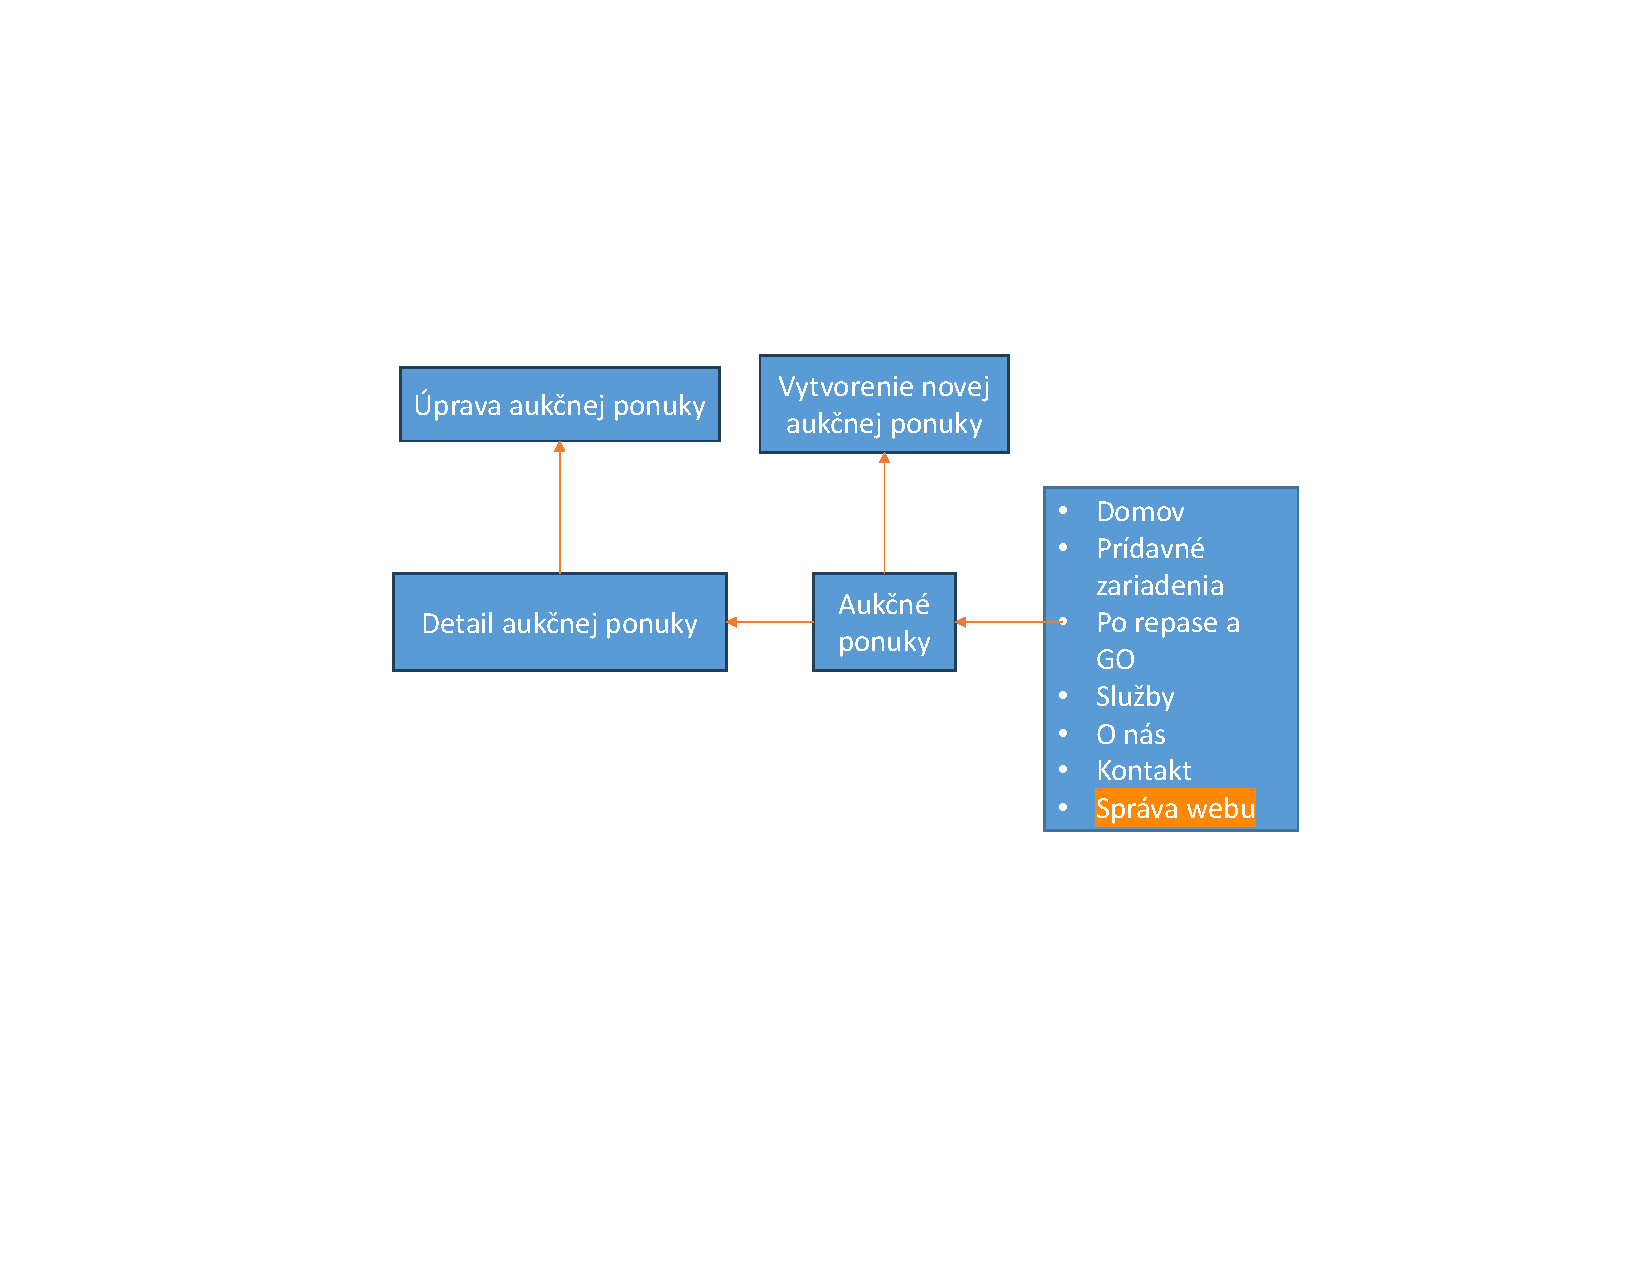
\includegraphics[width=140mm]{../img/UI concept/p4 graph}
\caption{Prechádzanie medzi časťami aplikácie spĺňajúcimi požiadavku P4.}
\label{p4 graph}
\end{figure}

\subsection{Aukčné ponuky}

Kliknutím na~odkaz~,,Po repase a GO`` v~navigácii má byť užívateľ presmerovaný do~časti aplikácie s~vylistovanými kartami aukčných ponúk (viď~obr.~\ref{auction offer cards}).

\begin{figure}[H]\centering
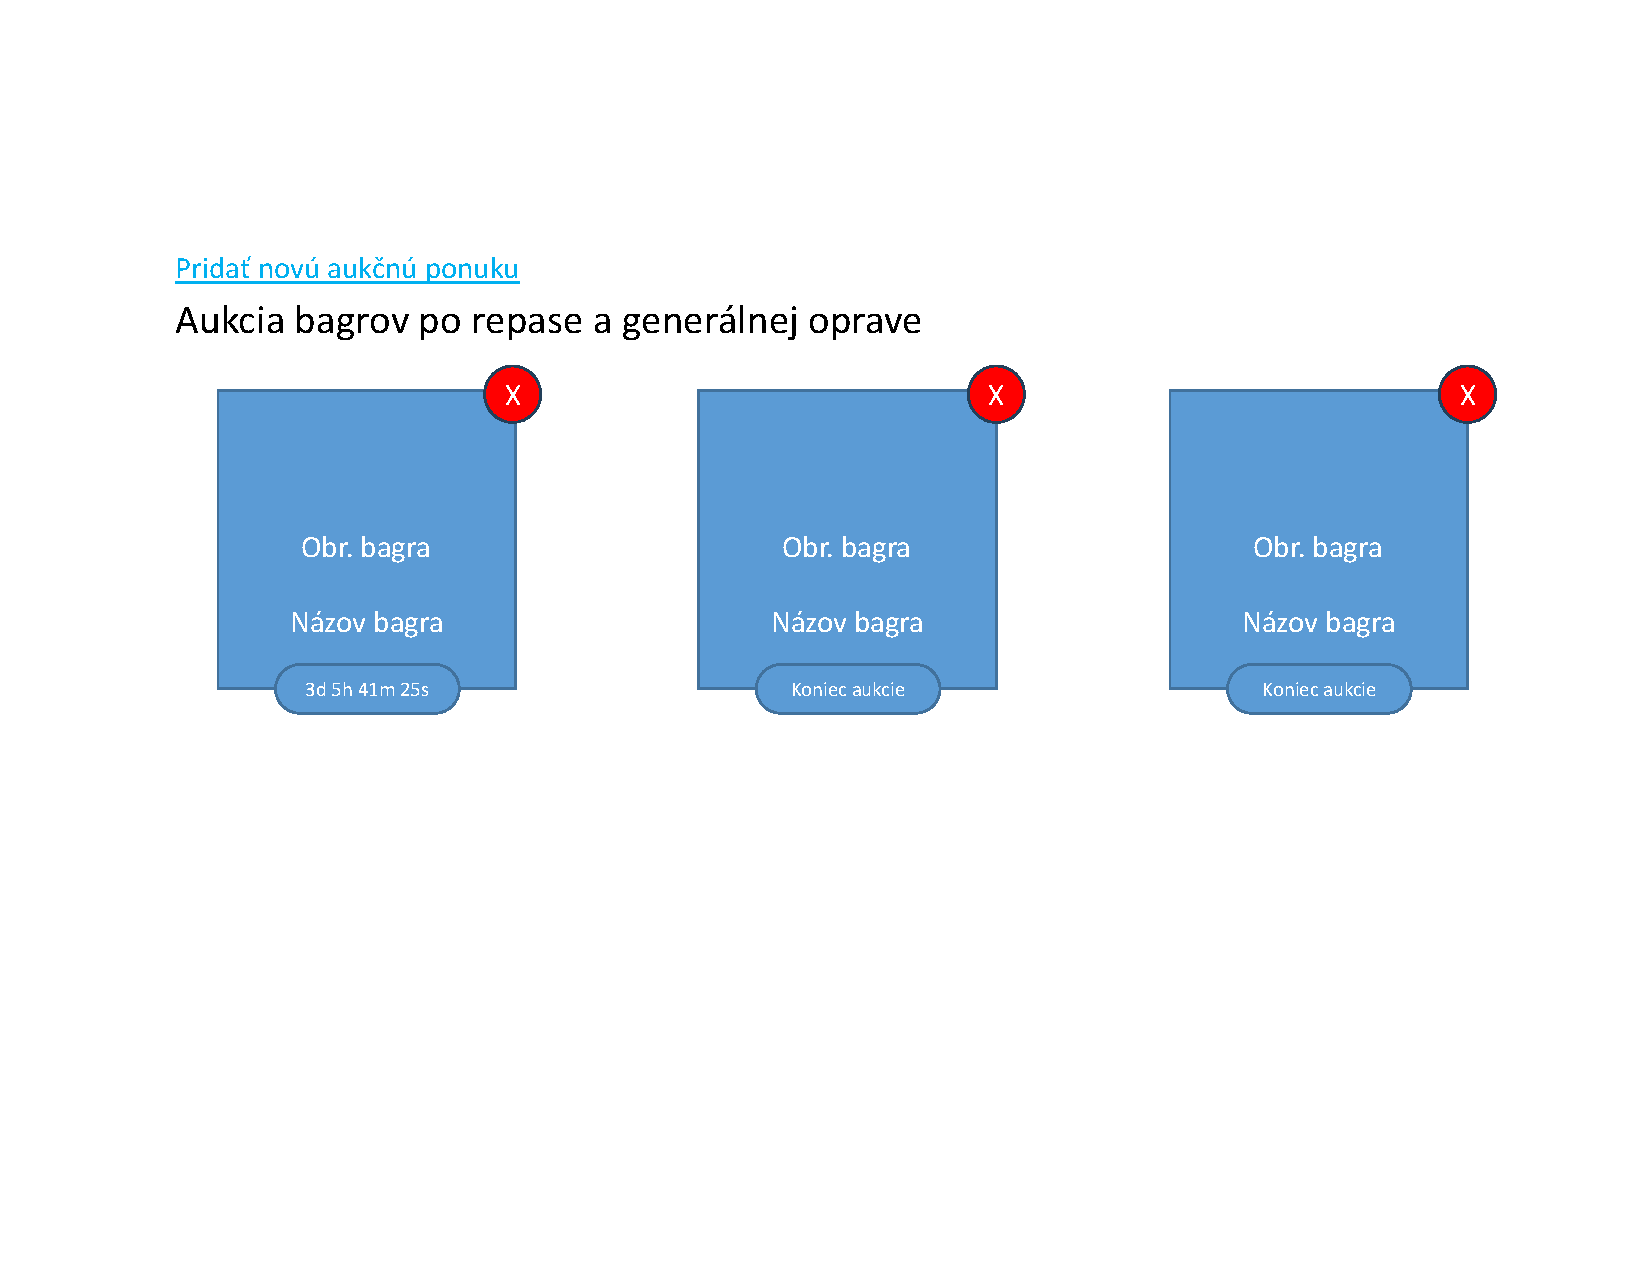
\includegraphics[width=140mm]{../img/UI concept/auction offer cards}
\caption{Aukčné ponuky.}
\label{auction offer cards}
\end{figure}

Karta aukčnej ponuky má obsahovať obrázok a~názov draženého bagra. V~spodnej časti sa má nachádzať odpočet do~konca dražby. Ďalej v~pravej hornej časti karty má byť tlačidlo~,,X``, viditeľné iba pre~adminsitrátora, ktorým môže ponuku vymazať. Po~kliknutí naň sa má zobraziť modálne potvrdzovacie okno s~nadpisom~,,Vymazať aukčnú ponuku natrvalo`` a~textom ,,Naozaj chcete túto aukčnú ponuku vymazať natrvalo?``.

Nad~kartami sa má nachádzať nadpis~,,Aukcia bagrov po~repase a~generálnej oprave``, a~takisto sa má vo~vrchnej časti nachádzať aj odkaz~,,Pridať novú aukčnú ponuku``, viditeľný iba pre~administrátorov, ktorý po~kliknutí presmeruje administrátora do~časti aplikácie, kde môže vytvoriť novú aukčnú ponuku.

Po~kliknutí na~nejakú z~kariet má byť užívateľ presmerovaný na~detail vybranej aukčnej ponuky.

\subsection{Detail aukčnej ponuky}

Po~kliknutí na~nejakú z~kariet aukčnej ponuky má byť užívateľ presmerovaný do~časti detailu aukčnej ponuky (viď~obr.~\ref{auction offer detail}).

\begin{figure}[H]\centering
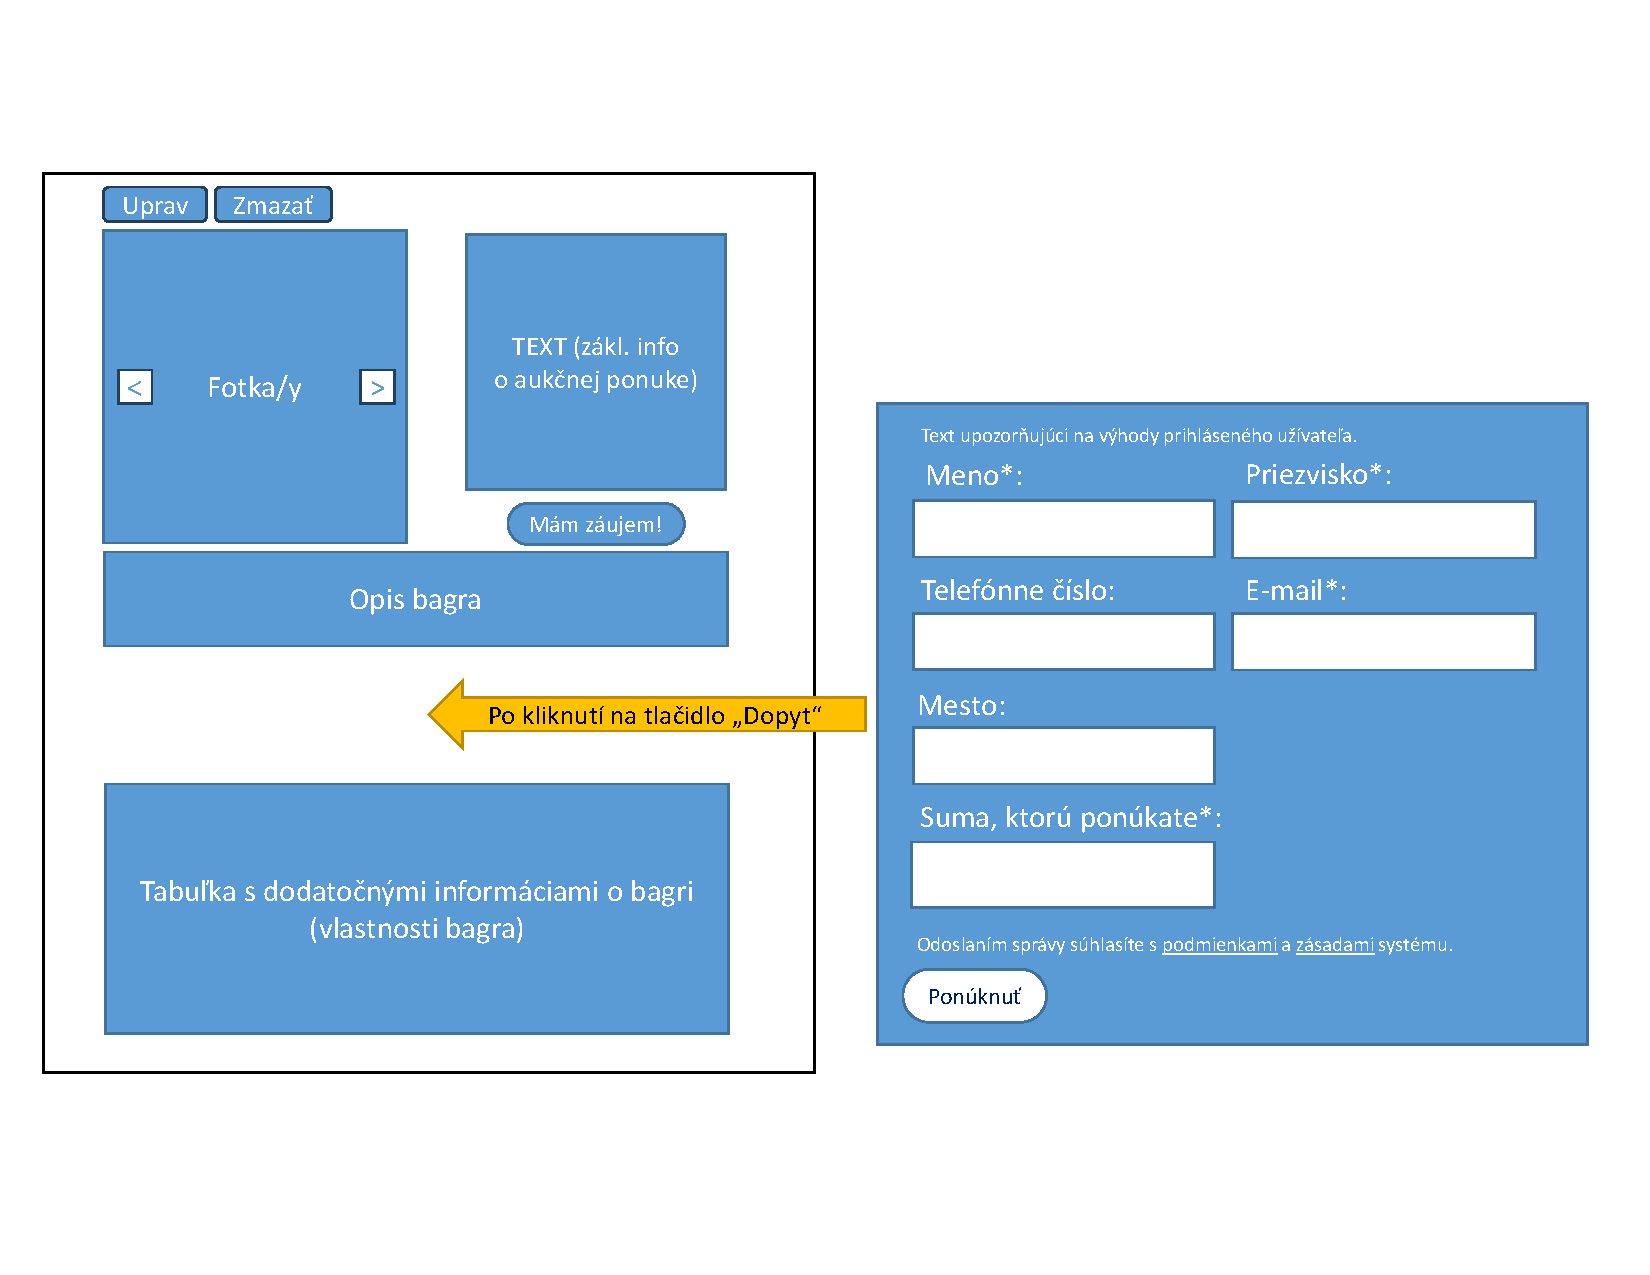
\includegraphics[width=140mm]{../img/UI concept/auction offer detail}
\caption{Detail aukčnej ponuky.}
\label{auction offer detail}
\end{figure}

V~tejto časti sa majú nachádzať fotky draženého bagra (klikaním na~tlačidlá šipiek vpravo, vľavo sa má prechádzať medzi fotkami predmetu). Ďalej sa majú v~tejto časti aplikácie nachádzať základné informácie o~aukčnej ponuke bagra (napr.~aký je bager starý, čo na~ňom bolo opravované atď.), okrem toho by mal byť v~tejto časti aj všeobecný popis bagra (všeobecné informácie o~bagri, ktoré platia nezávislé od~toho, že bol opravovaný), ďalej by sa v~tejto časti mala nachádzať tabuľka s~vlastnosťami bagra (napr.~výška, šírka atď.).

Okrem toho sa má v~tejto časti ešte nachádzať tlačidlo~,,Mám záujem!``. Po~kliknutí naň sa má zobraziť formulár, ktorým bude môcť užívateľ ponúknuť sumu do~dražby. Po~opätovnom kliknutí na~tlačidlo sa má formulár zatvoriť. 

Tlačidlo (a~ani formulár) sa nemajú zobrazovať administrátorom.

V~hornej časti sa má nachádzať tlačidlo~,,Upraviť``, ktoré má byť viditeľné iba pre~administrátorov. Po~kliknutí naň má byť administrátor presmerovaný na~formulár danej aukčnej ponuky, ktorým ju môže upravovať. Okrem tlačidla~,,Upraviť`` sa v~hornej časti má nachádzať aj tlačidlo~,,Zmazať``, takisto viditeľné iba pre~adminsitrátora, ktorým vie danú aukčnú ponuku zmazať.

\subsection{Ponúkanie sumy do~dražby}
\label{ponukanie sumy do drazby}

V~predošlej časti textu bolo spomenuté, že v~detaile bagra alebo~prídavného zariadenia sa má nachádzať tlačidlo~,,Mám záujem!``, ktorým si bude môcť zákazník (nie administrátor) zobraziť (a~opätovným kliknutím schovať) formulár pre~ponúknutie sumy do~dražby daného bagra.

Formulár má pre~neprihláseného zákazníka obsahovať povinné polia meno, priezvisko, email, ponúkaná suma, a takisto nepovinné polia telefón, mesto. Pre~prihláseného zákazníka má formulár obsahovať iba povinné pole ponúkaná suma. Povinné polia majú byť označené hviezdičkou. Navyše má platiť, že prvá zákazníkom ponúknutá suma môže byť rovná počiatočnej sume, ale nasledujúce ponúkané sumy musia mať medzi sebou rozdiel aspoň 100~eur.

Okrem polí má v~sebe formulár obsahovať pre~neprihlásených zákazníkov správu upozorňujúcu na~to, že prihlásený užívateľ nemusí vypĺňať svoje osobné údaje. Takisto by mal formulár pre~neprihláseného užívateľa obsahovať upozornenie, že s~odoslaním správy súhlasy s~podmienkami a~zásadami aplikácie.

Ďalej má formulár obsahovať tlačidlo~,,Ponúknuť``, ktoré má zákazníkovi umožniť ponúknutie sumy do~dražby o~daný bager.

Ak sú po~kliknutí na~tlačidlo~,,Ponúknuť`` povinné údaje nevyplnené alebo sú ich hodnoty neplatné, tak má na~to aplikácia užívateľa upozorniť chybovými správami pri~jednotlivých poliach.

Pre~lepšiu predstavu formulára viď~pravú časť obrázka~\ref{auction offer detail}.

\subsection{Vytvorenie novej a úprava existujúcej aukčnej ponuky}

Kliknutím na~odkaz~,,Pridať novú aukčnú ponuku``, ktorý sa má nachádzať v~časti s~vylistovanými aukčnými ponukami, má byť administrátor presmerovaný do~časti aplikácie, kde bude môcť vytvoriť novú aukčnú ponuku.

Podobne kliknutím na~tlačidlo~,,Upraviť``, ktoré sa má nachádzať v~časti s~detailom aukčnej ponuky, má byť administrátor presmerovaný do~časti aplikácie, kde bude môcť danú aukčnú ponuku upravovať.

Časť aplikácie pre~vytváranie novej aukčnej ponuky, ale takisto aj časť pre~u\-pra\-vo\-va\-nie existujúcej aukčnej ponuky, majú obsahovať formulár umožňujúci vloženie počiatočnej (vyvolávacej) ceny draženého bagra, dátumu konca dražby, popisu (napr.~aké časti boli v~bagri opravované), a~takisto by mal formulár obsahovať možnosť výberu stroja do~dražby. Údaj o~type bagra je povinný, dátum konca dražby nesmie obsahovať dátum v~minulosti a~počiatočná cena nesmie byť záporná.

Formulár má taktiež obsahovať tlačidlo~,,Reset`` na~vyprázdenie formulára.

Okrem tlačidla~,,Reset`` má obsahovať aj tlačidlo ,,Uložiť`` (na~uloženie aukčnej ponuky) ak sa vytvára nová aukčná ponuka alebo upravuje existujúca aukčná ponuka, ktorá je ešte stále aktívna (t.~j.~stále prebieha dražba). V prípade, že administrátor upravuje existujúcu aukčnú ponuku, ktorá už nie je aktívna, pretože stroj bol vydražený, tak sa má zobraziť tlačidlo~,,Uložiť a~spustiť odznova``. Toto správanie je vyžadované z~toho dôvodu, že ak výherca dražby z~nejakého dôvodu nebude súhlasiť s~prevzatím bagra, tak administrátor bude môcť celú dražbu odštartovať znova kliknutím na~tlačidlo~,,Uložiť a~spustiť odznova``.

Ak sú pri ukladaní povinné údaje nevyplnené alebo sú ich hodnoty neplatné, tak má na~to systém administrátora upozorniť prostrednictvom chybových správ pri~jednotlivých poliach.

Navyše nad~formulárom má byť v~prípade vytvárania novej aukčnej ponuky nadpis ,,Aukčné ponuky~-- vytvorenie nového záznamu`` a~v~prípade úpravy existujúcej aukčnej ponuky má byť nadpis ,,Aukčné ponuky~-- úprava existujúceho záznamu``.

Pre~lepšiu predstavu viď~obr.~\ref{auction offer form}.

\begin{figure}[H]\centering
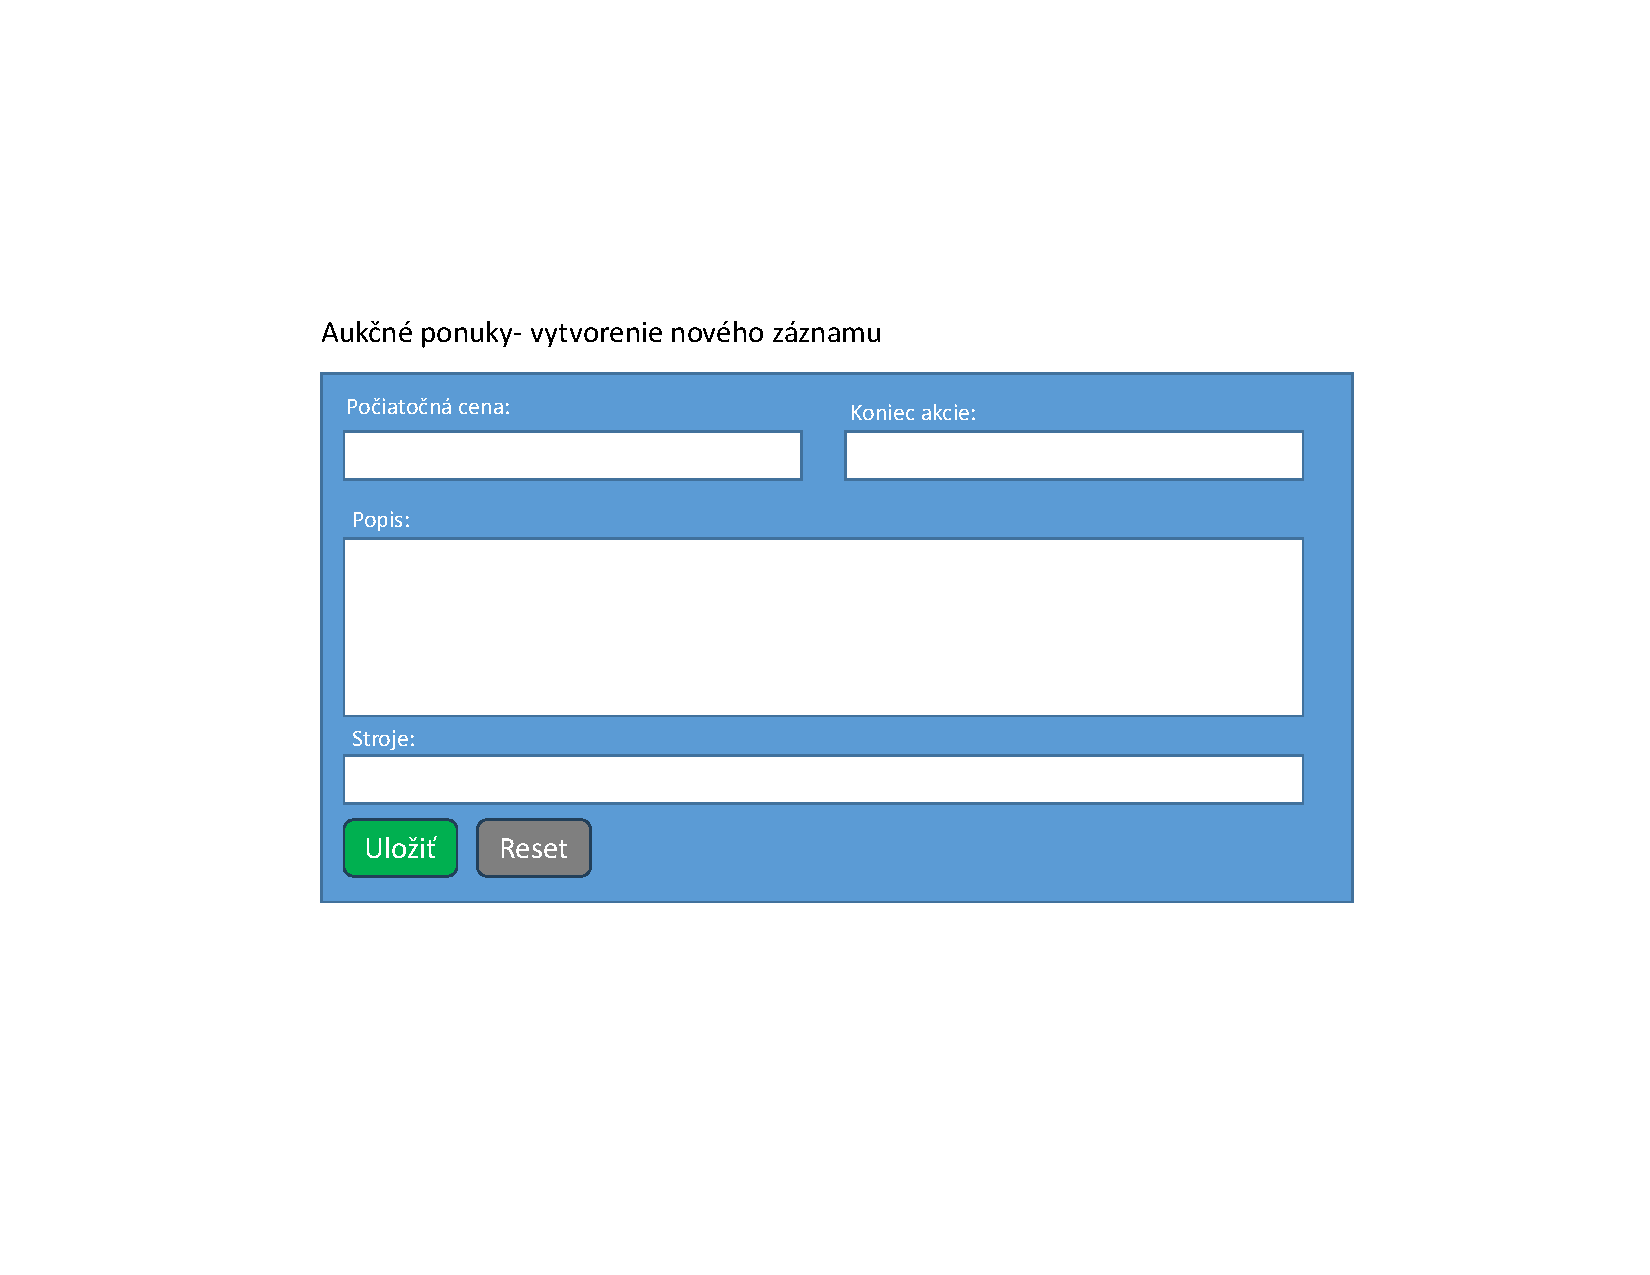
\includegraphics[width=140mm]{../img/UI concept/auction offer form}
\caption{Časť aplikácie pre~vytvorenie aukčnej ponuky.}
\label{auction offer form}
\end{figure}

\section{Splnenie P8}
\label{splnenie p8}

Po~kliknutí na~odkaz~,,Služby`` v~navigácii má byť užívateľ presmerovaný do~časti aplikácie, kde budú opísané výkopové služby, ktoré firma ponúka, a~tiež sa má v~tejto časti nachádzať tlačidlo~,,Mám záujem o~službu!``, ktoré nemá byť viditeľné pre~administrátorov. Pre lepšiu predstavu prechodu medzi časťami aplikácie viď~obr.~\ref{p8 graph}.

\begin{figure}[H]\centering
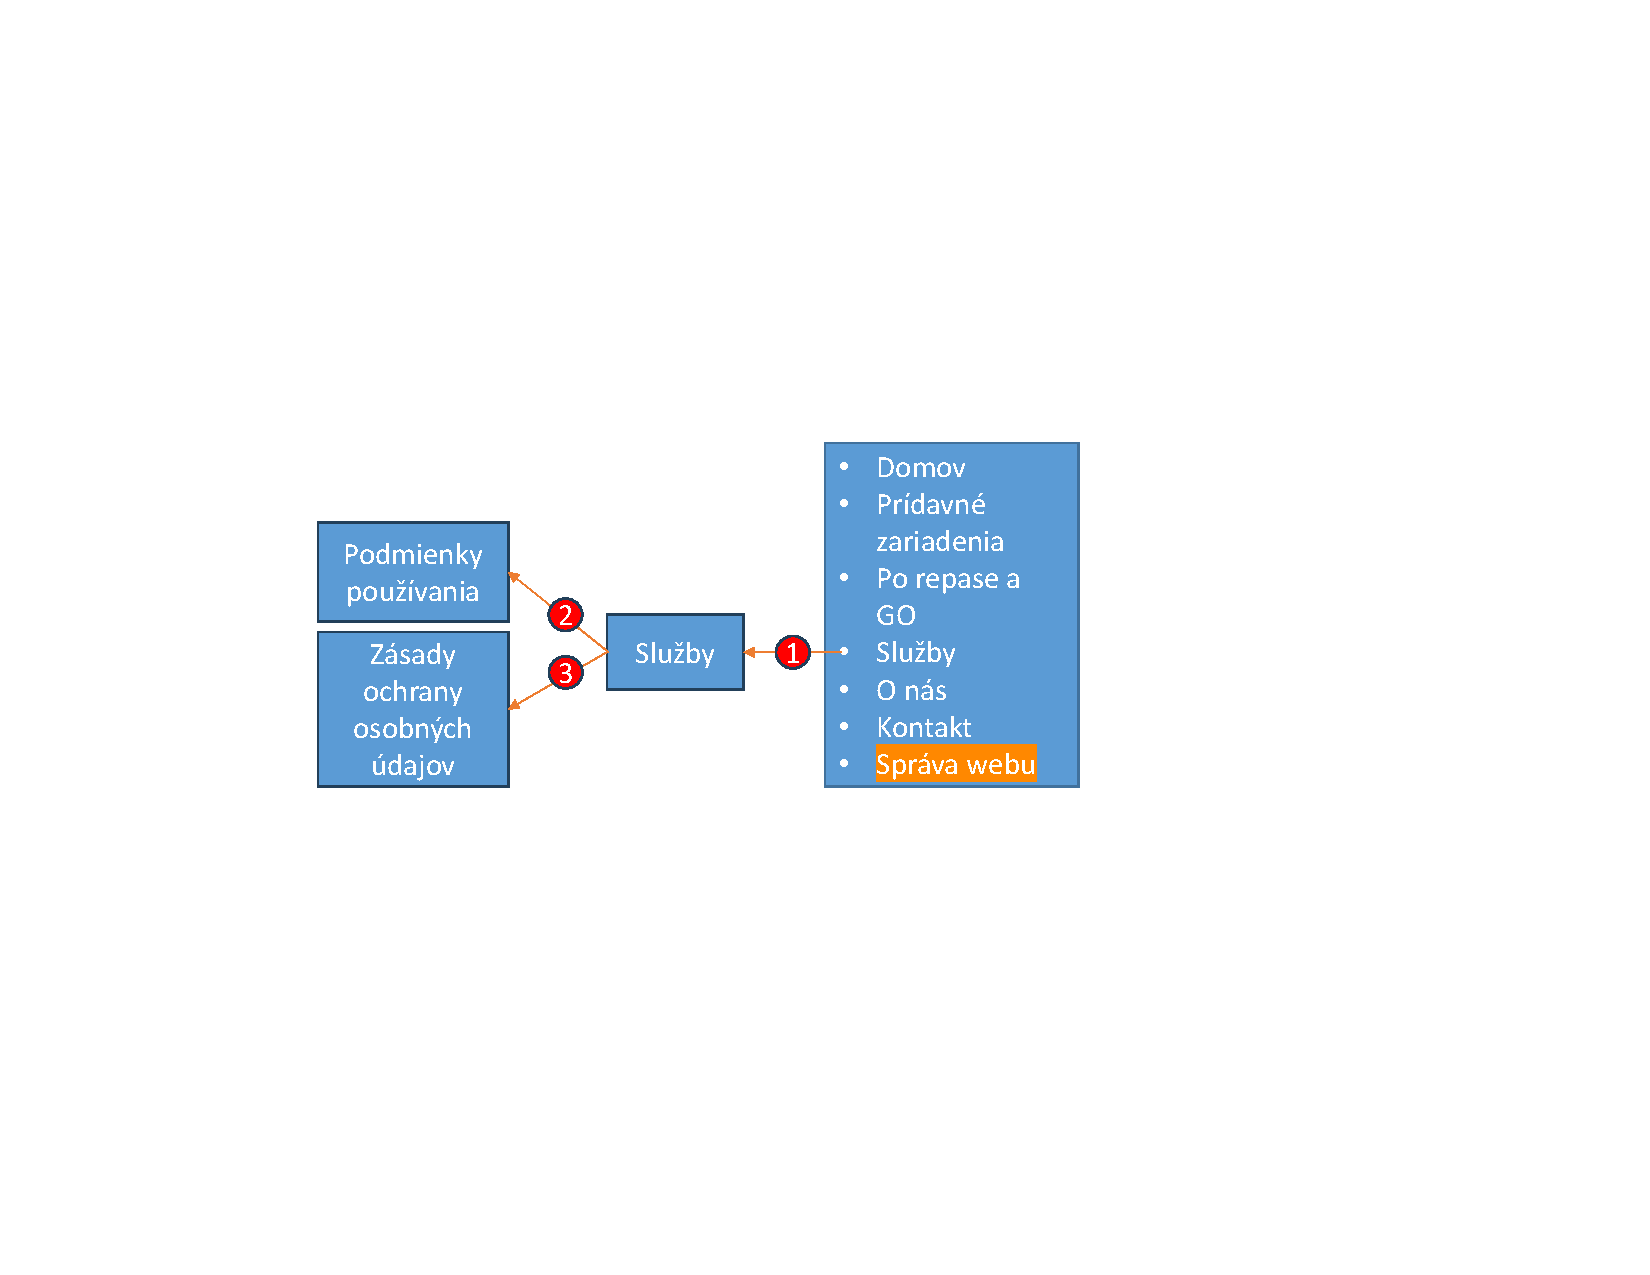
\includegraphics[width=140mm]{../img/UI concept/p8 graph}
\caption{Prechádzanie medzi časťami aplikácie spĺňajúcimi požiadavku~P8.}
\label{p8 graph}
\end{figure}

Kliknutím na~tlačidlo~,,Mám záujem o~službu!`` sa má zobraziť formulár, ktorým bude môcť užívateľ požiadať o~výkopovú službu. Opätovným kliknutím na~tlačidlo sa má formulár schovať.

Formulár má pre~neprihláseného zákazníka obsahovať povinné polia meno, priezvisko, email, správa, a~takisto nepovinné polia telefón, mesto. Pre~prihláseného zákazníka má formulár obsahovať iba povinné pole správa. Povinné polia majú byť označené hviezdičkou.

Okrem polí má v~sebe formulár obsahovať pre~neprihlásených zákazníkov správu upozorňujúcu na~to, že prihlásený užívateľ nemusí vypĺňať svoje osobné údaje. Takisto by mal formulár pre~neprihláseného užívateľa obsahovať upozornenie, že s~odoslaním správy súhlasí s~podmienkami a~zásadami aplikácie.

Ďalej má formulár obsahovať tlačidlo~,,Odoslať``, ktoré má zákazníkovi umožniť odoslanie žiadosti o~službu.

Ak sú po~kliknutí na~tlačidlo~,,Odoslať`` povinné údaje nevyplnené, tak má na~to aplikácia užívateľa upozorniť chybovými správami pri~jednotlivých poliach.

Pre~lepšiu predstavu opisovannej časti aplikácie a~formulára viď~obr.~\ref{services}.

\begin{figure}[H]\centering
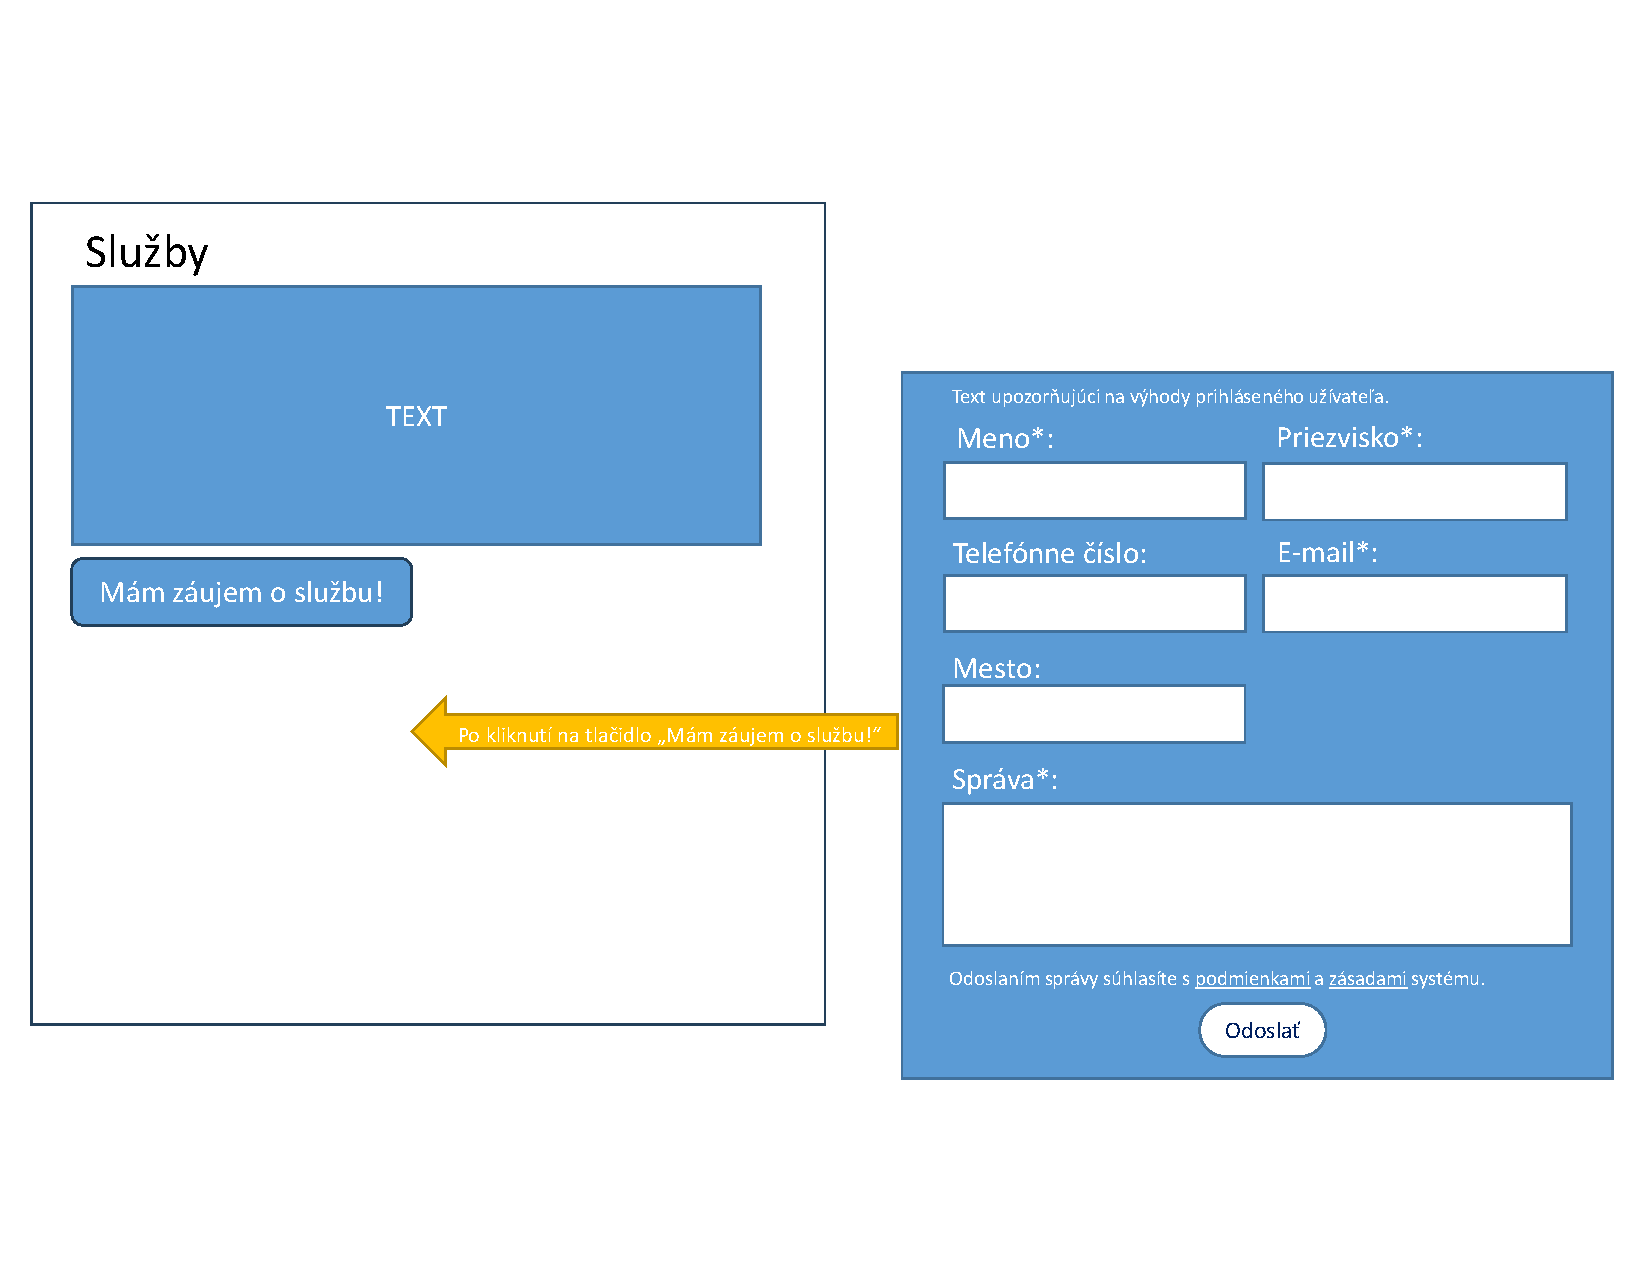
\includegraphics[width=140mm]{../img/UI concept/services}
\caption{Sekcia Služby.}
\label{services}
\end{figure}

\section{Splnenie P9}

Po~kliknutí na~odkaz~,,O~nás`` v~navigácii má byť užívateľ presmerovaný do~časti aplikácie, ktorá obsahuje text o~firme (napr.~jej histórii), príp. nejaké fotky.

Po~kliknutí na~odkaz~,,Kontakt`` v~navigácii alebo po~kliknutí na~telefónne číslo v hornej časti aplikácie (viď vpravo hore na obr.~\ref{layout}) má byť užívateľ presmerovaný do~časti aplikácie, ktorá obsahuje tabuľku s~kontaktom (telefónne číslo a~emailová adresa) firmy, príp.~aj iných pridružených firiem.

Pre~lepšiu predstavu prechodu medzi jednotlivými časťami aplikácie viď~obr.~\ref{p9 graph}.

\begin{figure}[H]\centering
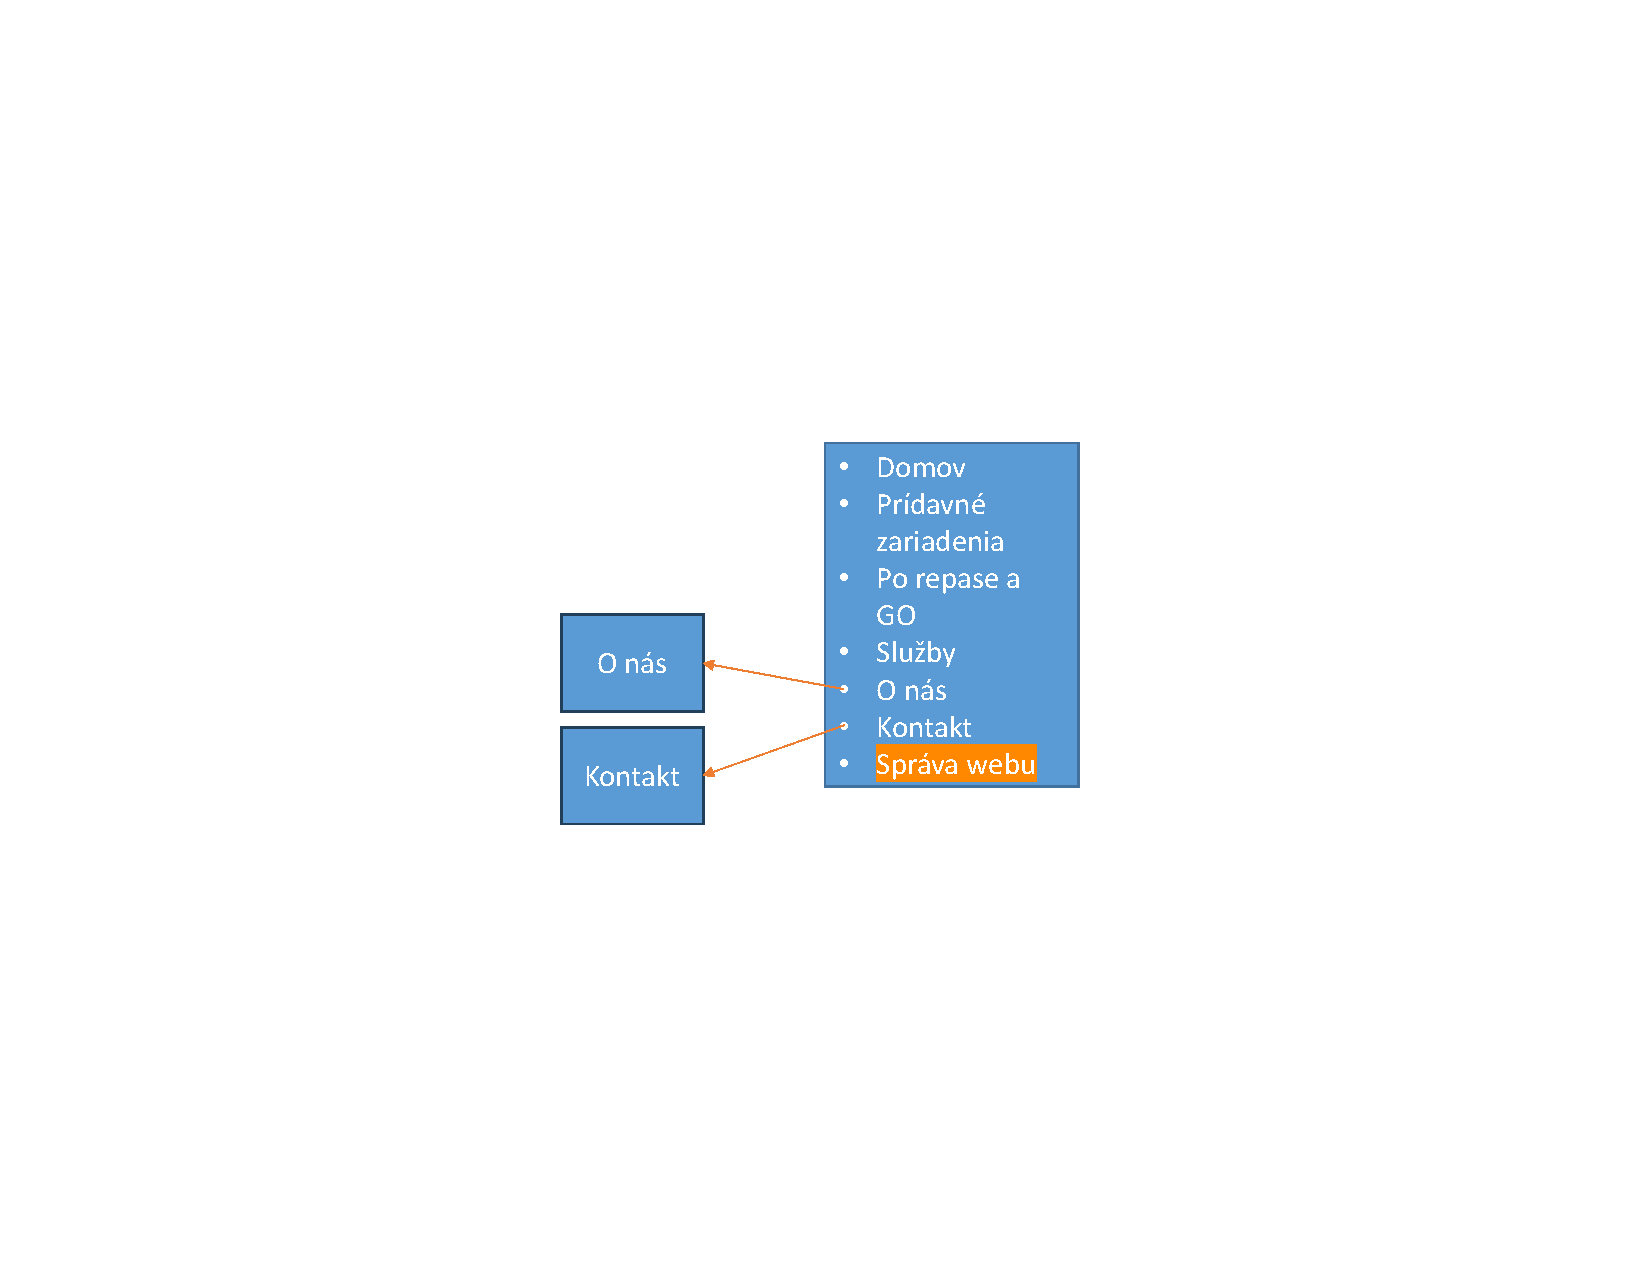
\includegraphics[width=140mm]{../img/UI concept/p9 graph}
\caption{Prechádzanie medzi časťami aplikácie spĺňajúcimi požiadavku~P9.}
\label{p9 graph}
\end{figure}

Pre~lepšiu predstavu sekcie~,,O~nás`` viď~obr.~\ref{about}.

\begin{figure}[H]\centering
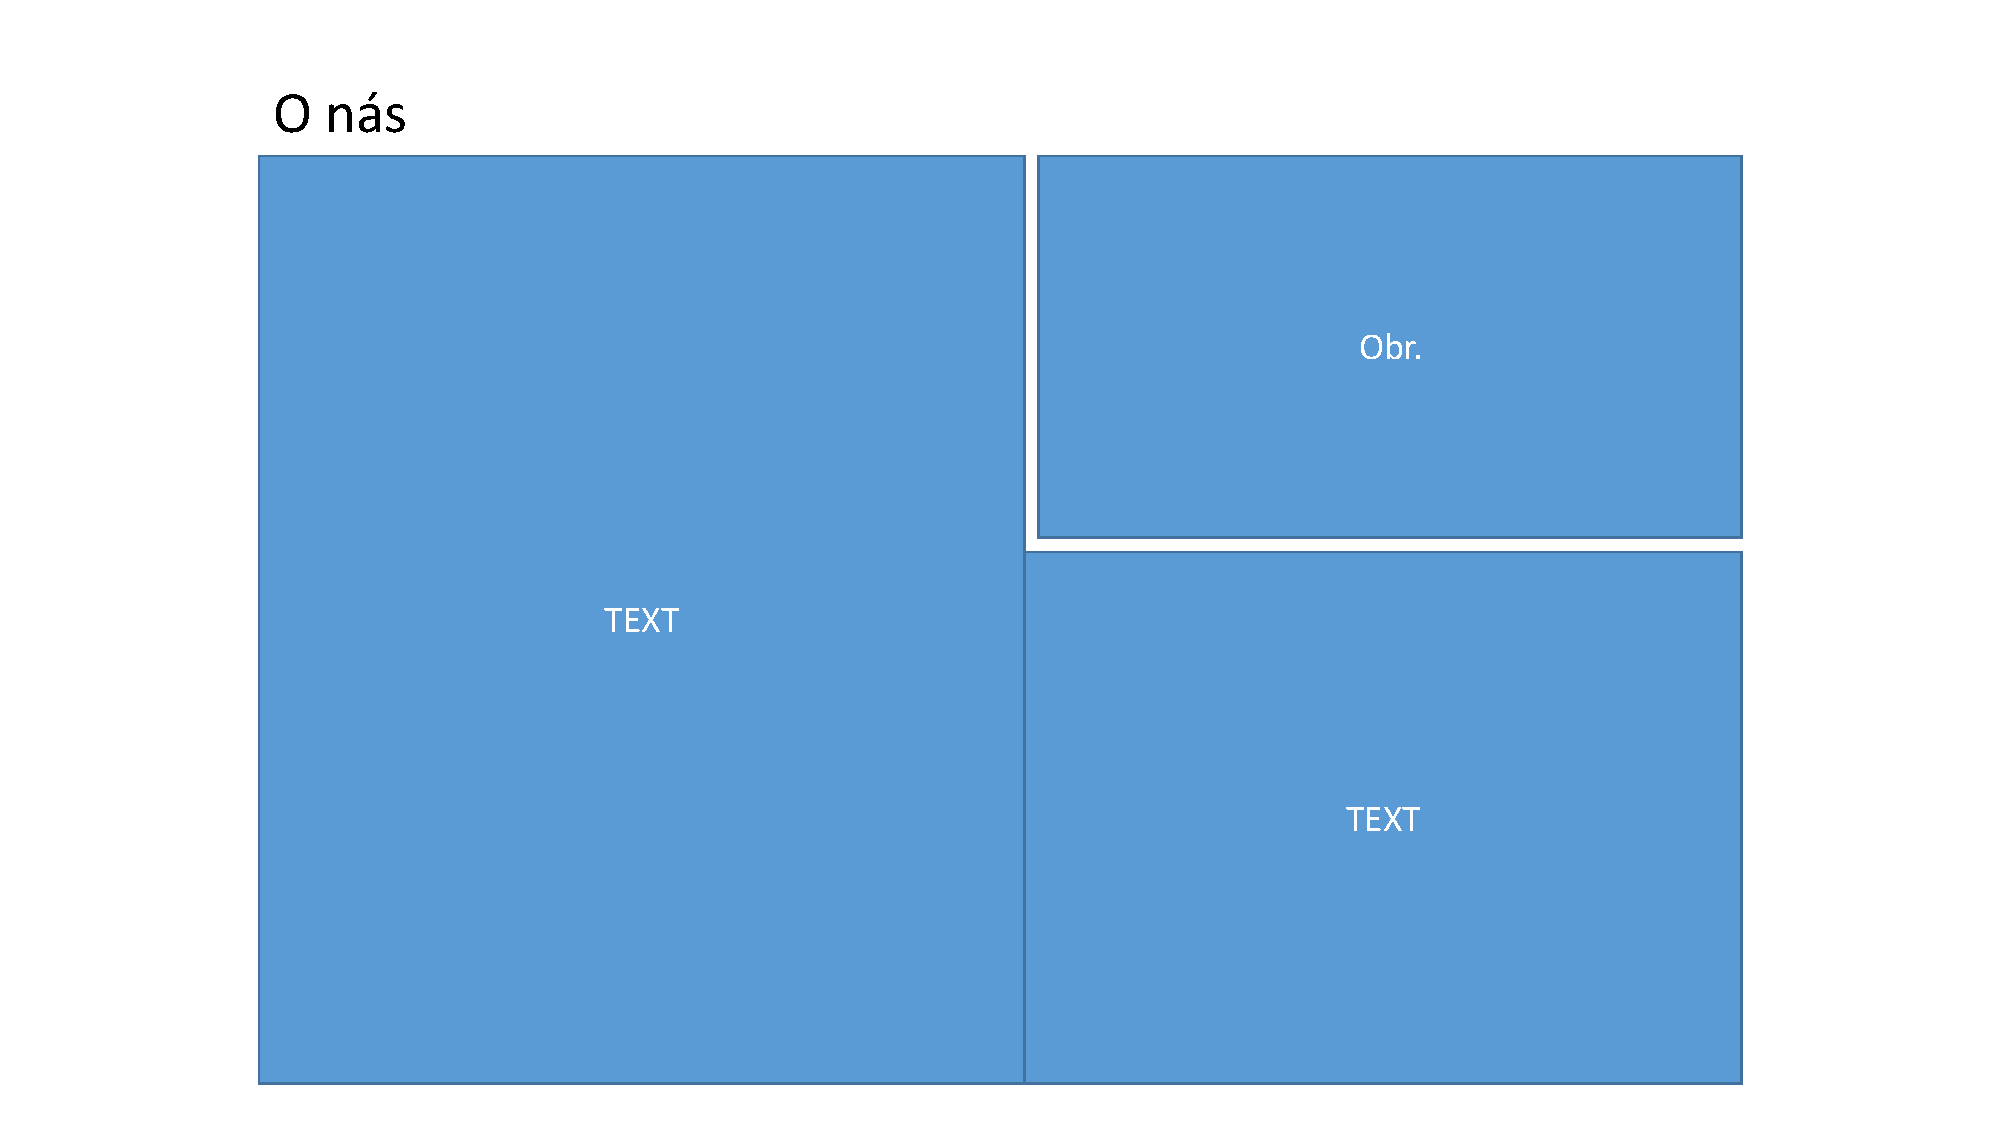
\includegraphics[width=140mm]{../img/UI concept/about}
\caption{Sekcia O~nás.}
\label{about}
\end{figure}

Pre~lepšiu predstavu sekcie~,,Kontakt`` viď~obr.~\ref{contact}.

\begin{figure}[H]\centering

\includegraphics[width=140mm]{../img/UI concept/contact}
\caption{Sekcia Kontakt.}
\label{contact}
\end{figure}

\section{Splnenie P5, P7 a~správa predmetov}
\label{splnenie p5 p7 a sprava predmetov}

Po~kliknutí na~odkaz~,,Správa webu`` v~navigácii, ktorý je viditeľný iba pre~administrátorov, má byť administrátor presmerovaný do~časti aplikácie, ktorá vyzerá následovne: v~hornej časti sa má nachádzať panel s~kartami, ktorými sa bude môcť administrátor preklikávať, a~pod~ním sa nachádza obsah podľa toho, na~akej karte sa administrátor nachádza.

Po príchode do tejto časti sa má administrátorovi zobraziť prvá karta~-- ,,Správy``. Okrem tejto karty sa bude môcť administrátor prekliknúť na karty: ,,Náhradné diely``, ,,Bagre``, ,,Typy bagrov``, ,,Typy vlastností bagrov``, ,,Kategórie a~značky bagrov``, ,,Kategórie a~značky prídavných zariadení``.

Na~karte~,,Správy`` majú byť vylistované konverzácie. Po~kliknutí na~nejakú z~konverzácií sa má administrátorovi zobraziť konverzácia. Ak bola konverzácia odoslaná z~našeho systému, má byť v~tejto konverzácii vložené prepojenie na~časť aplikácie z~ktorej bola správa odoslaná. Môže to byť buď detail bagra, detail prídavného zariadenia, detail aukčnej ponuky alebo~sekcia Služby.

Okrem toho sa má byť administrátor schopný dostať z~karty~,,Správy`` (pomocou tlačidla~,,Nastavenia``, ktore sa má na~karte nachádzať) do~časti aplikácie s~nastaveniami automaticky generovaných správ.

Pre~lepšiu predstavu prechodu medzi stránkami a~kartami viď~obr.~\ref{p5 p7 a sprava predmetov graph}.

\begin{figure}[H]\centering
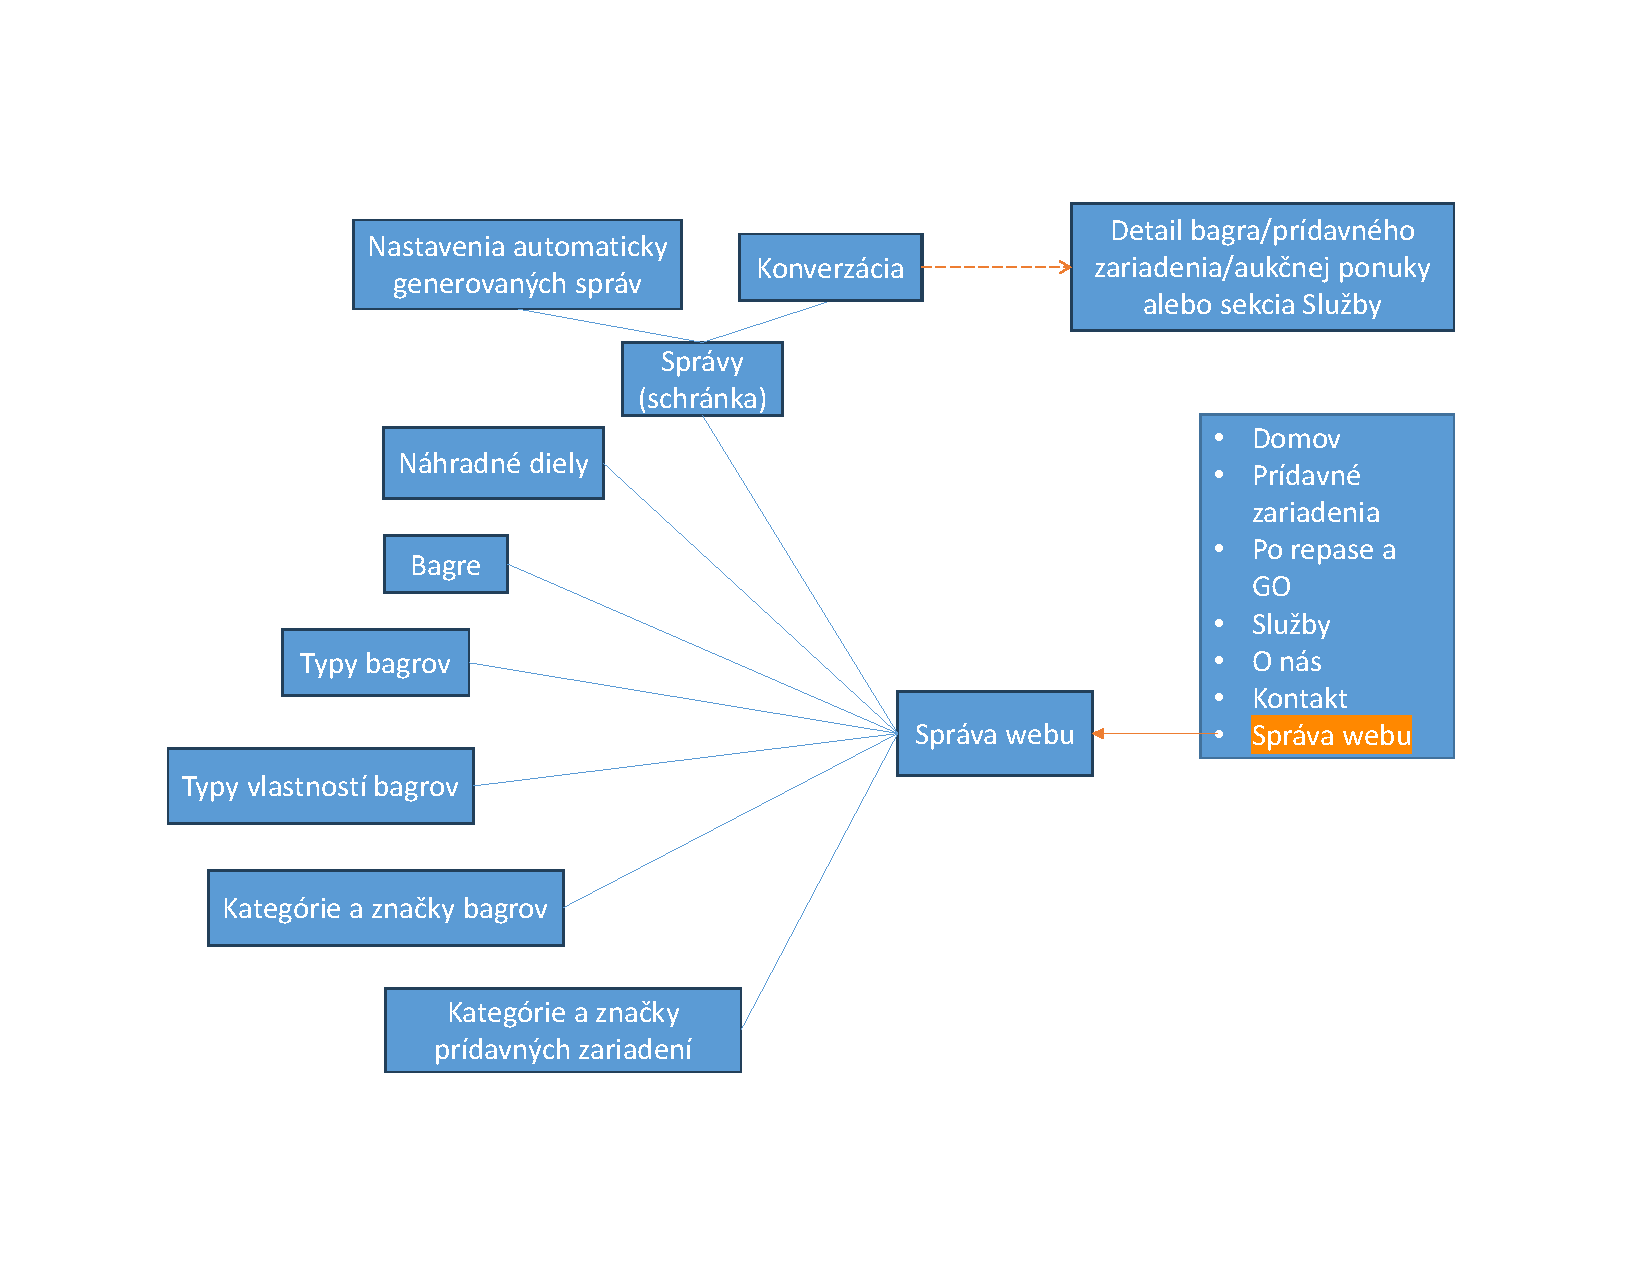
\includegraphics[width=140mm]{../img/UI concept/p5 p7 a sprava predmetov graph}
\caption{Prechádzanie medzi časťami aplikácie spĺňajúcimi požiadavku P5 (orientovaná hrana značí prechod do~novej časti aplikácie, neorientovaná prepínanie medzi časťami, prerušovaná nepovinný prechod do~novej časti).}
\label{p5 p7 a sprava predmetov graph}
\end{figure}

\subsection{Správy~-- schránka}

Po~príchode do~sekcie~,,Správa webu`` alebo po~kliknutí na~kartu~,,Správy`` v~sekcii~,,Správa webu`` sa má administrátorovi zobraziť emailová schránka podobná Gmailu (viď~obr.~\ref{messages}).

\begin{figure}[H]\centering
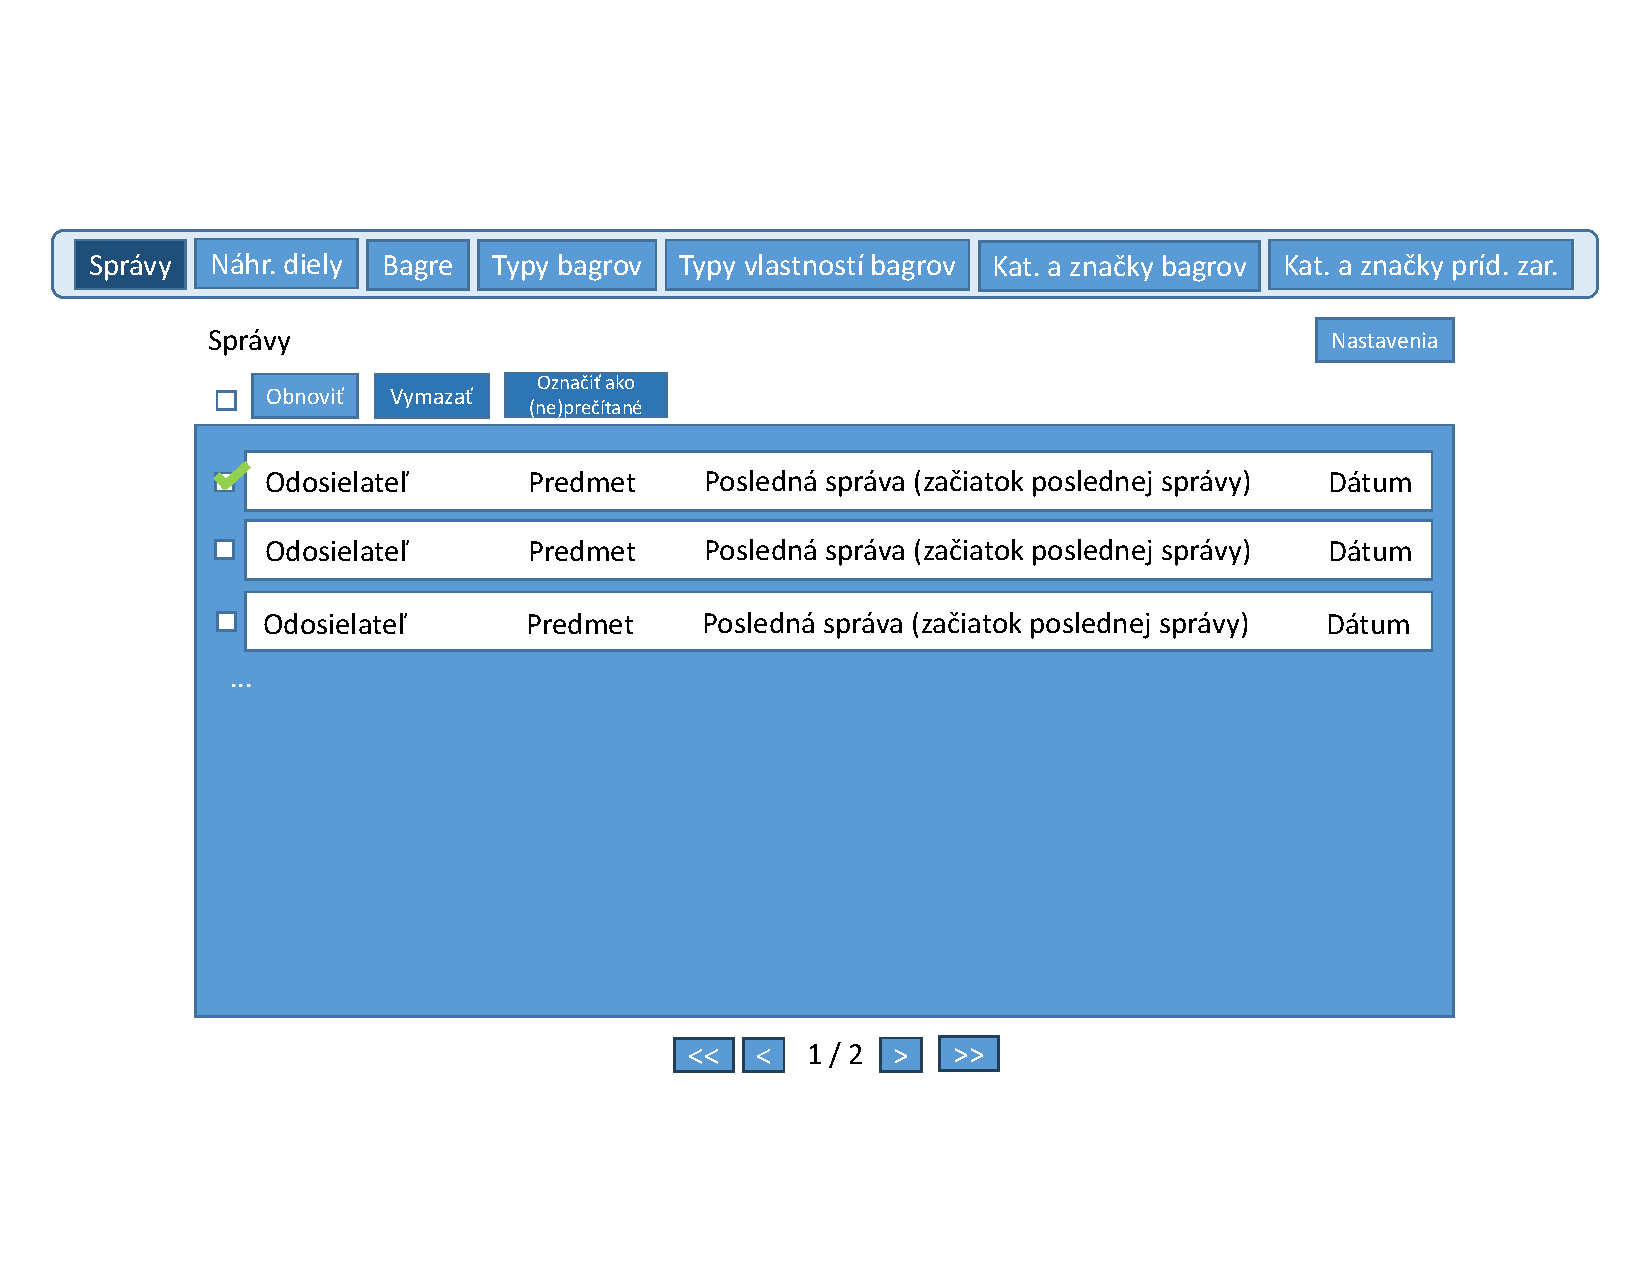
\includegraphics[width=140mm]{../img/UI concept/messages}
\caption{Emailová schránka}
\label{messages}
\end{figure}

V~schránke majú byť vylistované konverzácie (vlákna správ) zhora dole od~najnovšej po+najstrašiu. Každá takáto konverzácia má byť reprezentovaná riadkom, v~ktorom je uvedené meno odosielateľa, predmet, a~text poslednej správy (resp.~jeho začiatok v~prípade dlhšieho textu) a~dátum poslednej správy (emailu v~konverzácii).

Vylistované konverzácie by mali byť stránkované (max.~osem konverzácii na~stránku). Pod~vylistovanými konverzáciami by malo byť tlačidlo~,,<<``, ktoré presunie administrátora na prvú stranu vylistovaných konverzácií, tlačidlo~,,<``, ktoré presunie administrátora o~jednu stranu dopredu (ak ešte nie je na~prvej stran) a~tlačidlá~,,>``, ,,>>``, ktoré majú fungovať analogicky (lenže na~opačnú stranu).

Veľa každého riadka konverzácie má byť začiarkovacie políčko, ktorým vieme konverzáciu označiť.

Nad~vylistovanými konverzáciami má byť nadpis~,,Správy`` a~tlačidlo~,,Nastavenia``, ktorým sa bude môcť administrátor dostať do~časti aplikácie s~nastaveniami automaticky generovaých správ. 

Ďalej pod~nadpisom má byť začiarkovacie políčko, ktorým bude môcť administrátor začiarknúť (označiť) všetky konverzácie na~aktuálnej strane. Okrem tohto začiarkovacieho políčka, tam majú byť tlačidlo~,,Obnoviť`` a~ak je označená aspoň jedna konverzácia, tak potom sú viditeľné aj tlačidlá~,,Vymazať`` a~,,Označiť ako prečítané`` alebo~,,Označiť ako neprečítané``.

Tlačidlo~,,Označiť ako neprečítané`` sa zobrazí vtedy, keď sú všetky označené správy prečítané. Tlačidlo~,,Označiť ako prečítané`` sa zobrazí vtedy, keď sú všetky označené správy neprečítané alebo sú medzi správami aj prečítané, aj neprečítané správy.

Tlačidlom~,,Vymazať`` bude môcť administrátor vymazať označené konverzácie. Po~kliknutí naň sa má zobraziť potvrdzovacie modálne okno s~nadpisom~,,Vymazať vybrané konverzácie`` a textom~,,Naozaj chcete vymazať vybrané konverzácie natrvalo?``.

Po~kliknutí na~nejaký z~riadkov sa má administrátorovi zobraziť vybraná konverzácia.

\subsection{Správy~-- konverzácia}

Po~kliknutí na~nejakú z~konverzácií sa má administrátorovi zobraziť daná konverzácia (viď~obr.~\ref{message}).

\begin{figure}[H]\centering
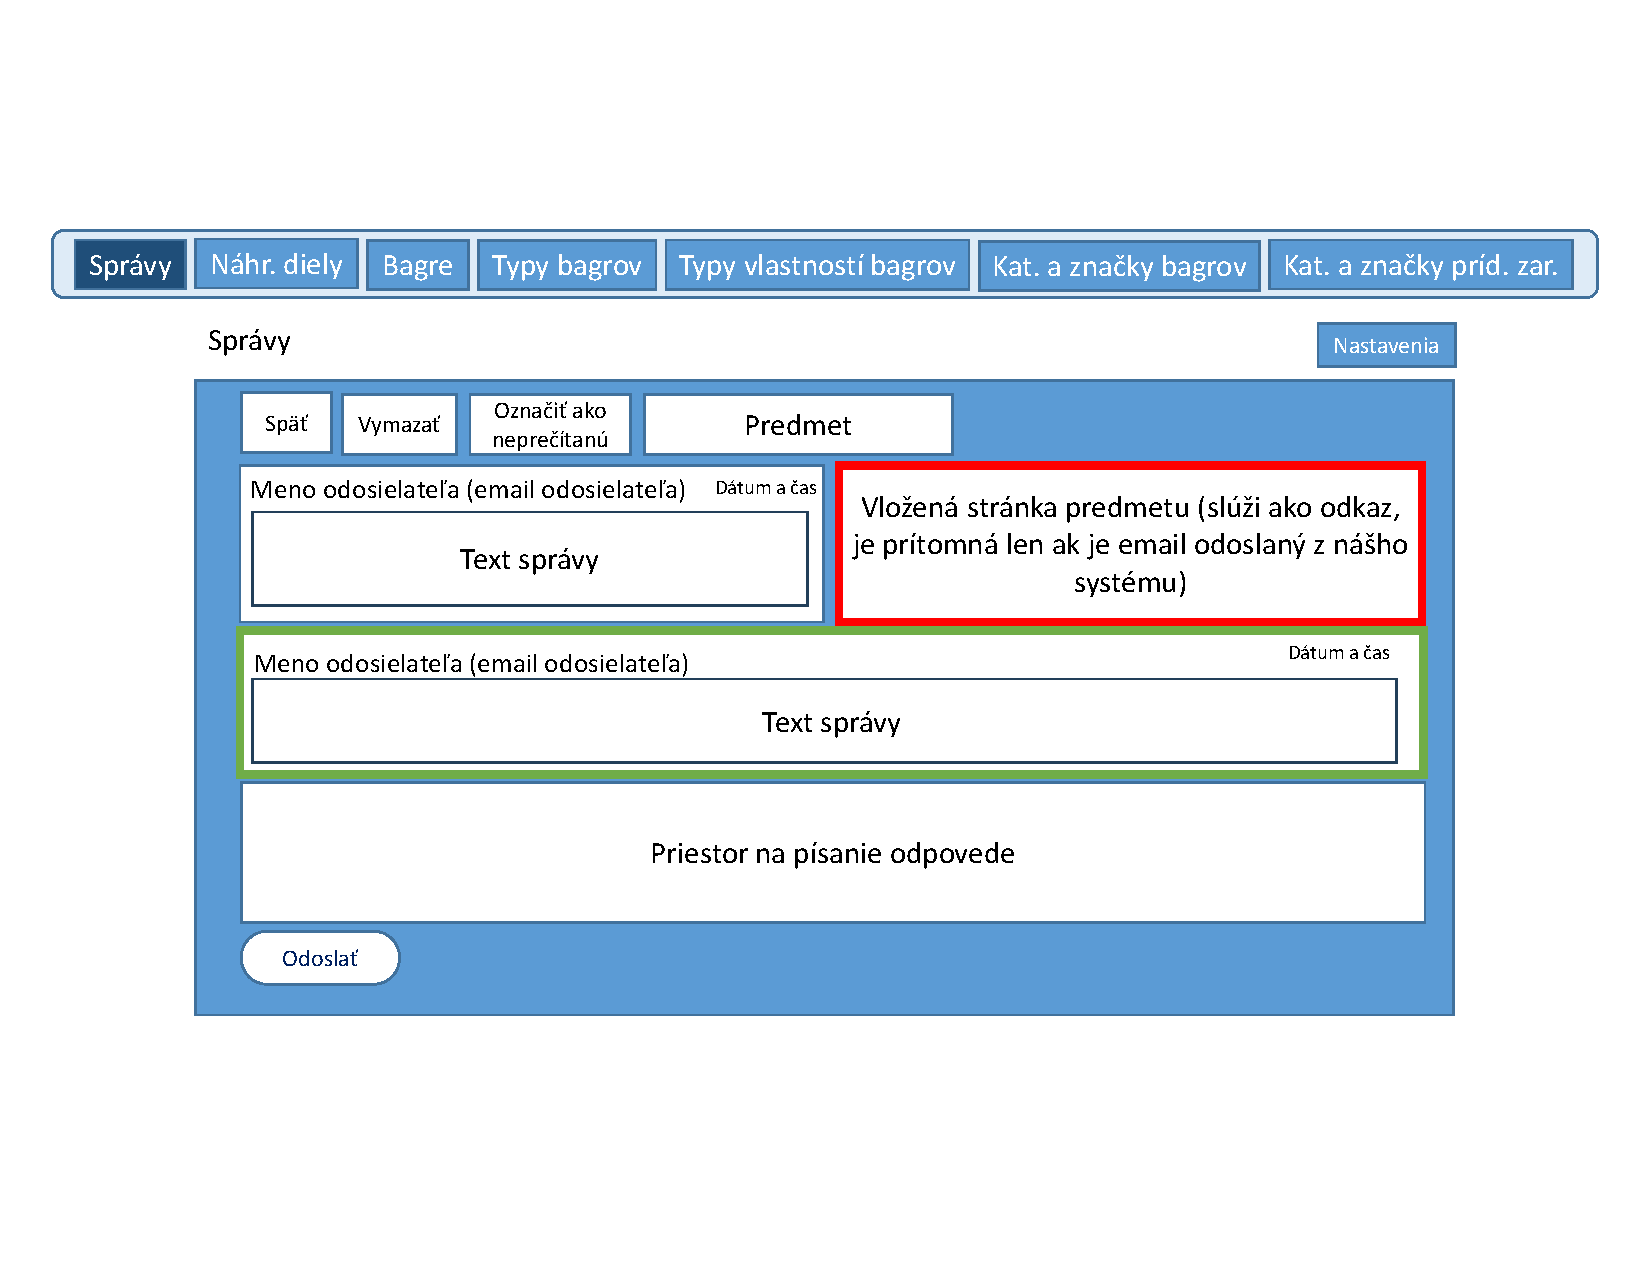
\includegraphics[width=140mm]{../img/UI concept/message}
\caption{Konverzácia}
\label{message}
\end{figure}

V hornej časti sa má nacházať nadpis~,,Správy`` a~tlačidlo~,,Nastavenia`` (pre~otvorenie nastavenia automaticky generovaných správ). Pod nimi sa majú nachádzať tlačidlá~,,Späť`` (pre~návrat do~schránky), ,,Vymazať`` a~tlačidlo~,,Označiť ako neprečítanú`` (pre~označenie správy za~neprečítanú).

Tlačidlom~,,Vymazať`` bude môcť administrátor vymazať otvorenú konverzáciu. Po~kliknutí sa má zobraziť potvrdzovacie modálne okno s~nadpisom~,,Vymazať konverzáciu`` a textom~,,Naozaj chcete vymazať túto konverzáciu natrvalo?``.

Napravo od~tlačidiel má byť zobrazený predmet (poslednej správy v konverzácii).

Pod~tlačidlami a~predmetom majú byť zobrazené jednotlivé správy~(emaily) konverzácie zoradené zhora dole od~najstaršej po~najnovšiu.

Ak bola (prvá) správa odoslaná z~nášho systému, tak vedľa nej má byť vložená časť aplikácie, odkiaľ bola správa odoslaná (na~obr.~\ref{message} viď~časť označenú červeným rámom). Po~kliknutí na~túto časť má byť administrátor presmerovaný do~časti aplikácie, odkiaľ bola správa odoslaná (má sa otvoriť v~novom okne). V prípade, že správa nebola odoslaná z nášho systému, má sa správa roztiahnuť na~šírku tejto časti aplikácie (rovnako ako je druhá správa, označená zeleným rámom, na~obr.~\ref{message}).

Pre~každú správu v~konverzácii sa má zobraziť meno a~email odosielateľa, dátum a~čas správy, a~takisto text správy.

Pod~vylistovanými správami má byť priestor pre~písanie odpovede a~tlačidlo~,,Odoslať``, ktorým môže administrátor odosielať správy do~konverzácie.

\subsection{Správy~-- nastavenia automaticky generovaných správ}

Po~kliknutí na~tlačidlo~,,Nastavenia`` sa administrátorovi zobrazia nastavenia automaticky generovaných správ (viď~obr.~\ref{messages settings}).

\begin{figure}[H]\centering
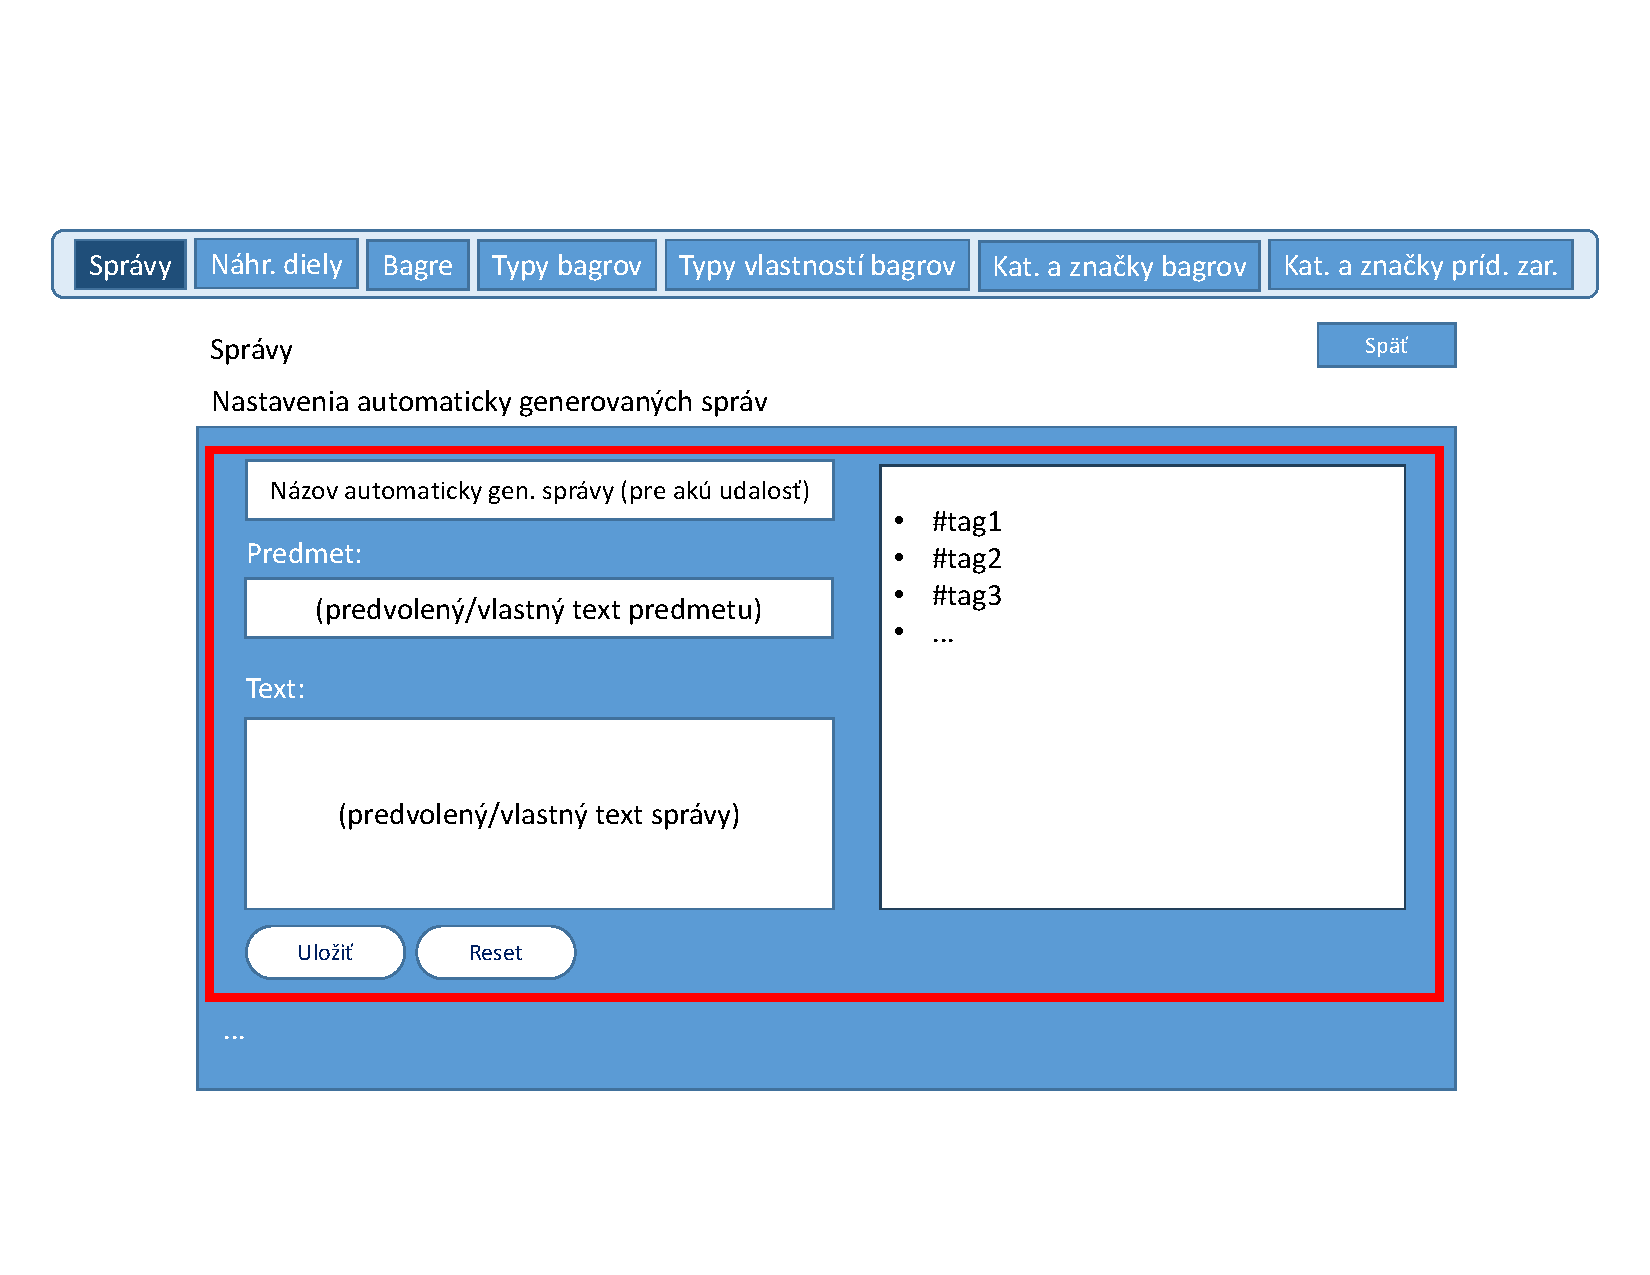
\includegraphics[width=140mm]{../img/UI concept/messages settings}
\caption{Nastavenia automaticky generovaných správ}
\label{messages settings}
\end{figure}

Vo~vrchnej časti sa má nachádzať nadpis~,,Správy`` a~tlačidlo~,,Späť``, ktoré schová/zatvorí nastavenia. Pod~nimi sa má nachádzať nadpis~,,Nastavenia automaticky generovaných správ`` a~sekcia, kde sa pre~každú automaticky generovanú správu zobrazí časť, kde sa dá nastavovať jej tvar (jedna zo~spomínaných častí je vyznačená červeným rámom na~obr. \ref{messages settings}).

Každá z~takýchto častí má obsahovať názov automaticky generovanej správy (resp.~pre koho, akú udalosť je určená, napr.~,,Pre~víťaza aukcie``). Ďalej má obsahovať šablónu predmetu, šablónu textu. A~v~pravej časti zoznam tagov povolených v~danej automaticky generovanej správe.

Tag má tvar ,,\#\{názov tagu\}``, kde názov tagu môže obsahovať iba písmená a~znak ,,\_``. Pomocou tagov bude vedieť administrátor špecifikovať kde sa má v~texte (reps. predmete) automaticky generovanej správy nachádzať konkrétna hondota špecifikovaná tagom. Napr.~ak by sme použili vetu~,,Gratulujeme, vyhrali ste \#nazov\_stroja`` ako šablónu predmetu, tak email, ktorý by prišiel užívateľovi by mohol vyzerať takto:~,,Gratulujeme, vyhrali ste Stroj123`` (ak by bol názov výherného stroja ,,Stroj123``).

Každá z~automaticky generovaných správ má mať predvolený text, ktorý bude môcť byť pomocou šablón prepísaný. Ak nebudú definované vlastné šablóny, majú sa využívať predvolené, a~preto sa majú v~spomínaných poliach pre~predmet a~text zobrazovať predvolené šablóny. Ak by boli predvolené šablóny prepísané a~neskôr sa vymažú, tak polia sa majú znova napĺniť predvolenými hodnotami.

Ďalej pod~poliami sa majú nachádzať tlačidlá~,,Uložiť`` (pre~uloženie šablón) a~,,Reset`` (pre~navrátenie k~predvoleným hodnotám).

\subsection{Náhradné diely}

TODO

\subsection{Bagre}

TODO?

\section{Splnenie P6}
\label{splnenie p6}

V~tejto podkapitole si prejdeme časti aplikácie spĺňajúce požiadavku P6, t.~j.~umožnenie užívateľom registrovať a~prihlásiť sa do~systému (pričom administrátori sa majú prihlasovať rovnakým spôsobom ako bežńi zákazníci), umožnenie zmeny údajov v~profile, zjednodušenie prihláseným užívateľom vypĺňanie formulárov (aby nemuslei zadávať svoje osobné údaje, umožnenie neprihláseným užívateľom posielať dopyty a~účastniť sa aukčných dražieb.

V~častaiach~\ref{dopyt}, \ref{ponukanie sumy do drazby} a~\ref{splnenie p8} už bolo spomenuté, že aj prihlásení, aj neprihlásení užívatelia sa môžu dopytovať na~bager, prídavné zariadenie, výkopovú službu alebo~takisto môžu ponúkať sumy do~dražby (teda zapájať sa do~aukcie). Pričom prihláseným užívateľom sa nemajú zobrazovať polia s osobnými údajmi, takže ich nemusia vypĺňať. Tým pádom sú požiadavky zjednodušenie vypĺňania formulárov prihlásenými užívateľmi, umožnenie posielania dopytov neprihláseným užívateľom a~umožnenie účasti v~aukcii neprihláseným užívateľom splnené.

\subsection{Prihlasovací panel}

V~ľavej časti aplikácie nad~navigáciou sa má nachádzať prihlasovací panel (pre~lepšiu predstavu umiestnenia panela viď~obr~\ref{layout})).

Ak je užívateľ neprihlásený, tak sa majú v~prihlasovacom paneli nachádzať tlačidlá~,,Prihlásiť`` a~,,Registrovať`` (viď~vľavo hore na~obr.~\ref{auth}).

Po~kliknutí na~tlačidlo~,,Prihlásiť`` má byť užívateľ presmerovaný do~časti aplikácie s~prihlasovacím formulárom (viď~ľavú časť obr.~\ref{auth}).

Po~kliknutí na~tlačidlo~,,Registrovať`` má byť užívateľ presmerovaný do~časti aplikácie s~registračným formulárom (viď~pravú časť obr.~\ref{auth}).

\begin{figure}[H]\centering
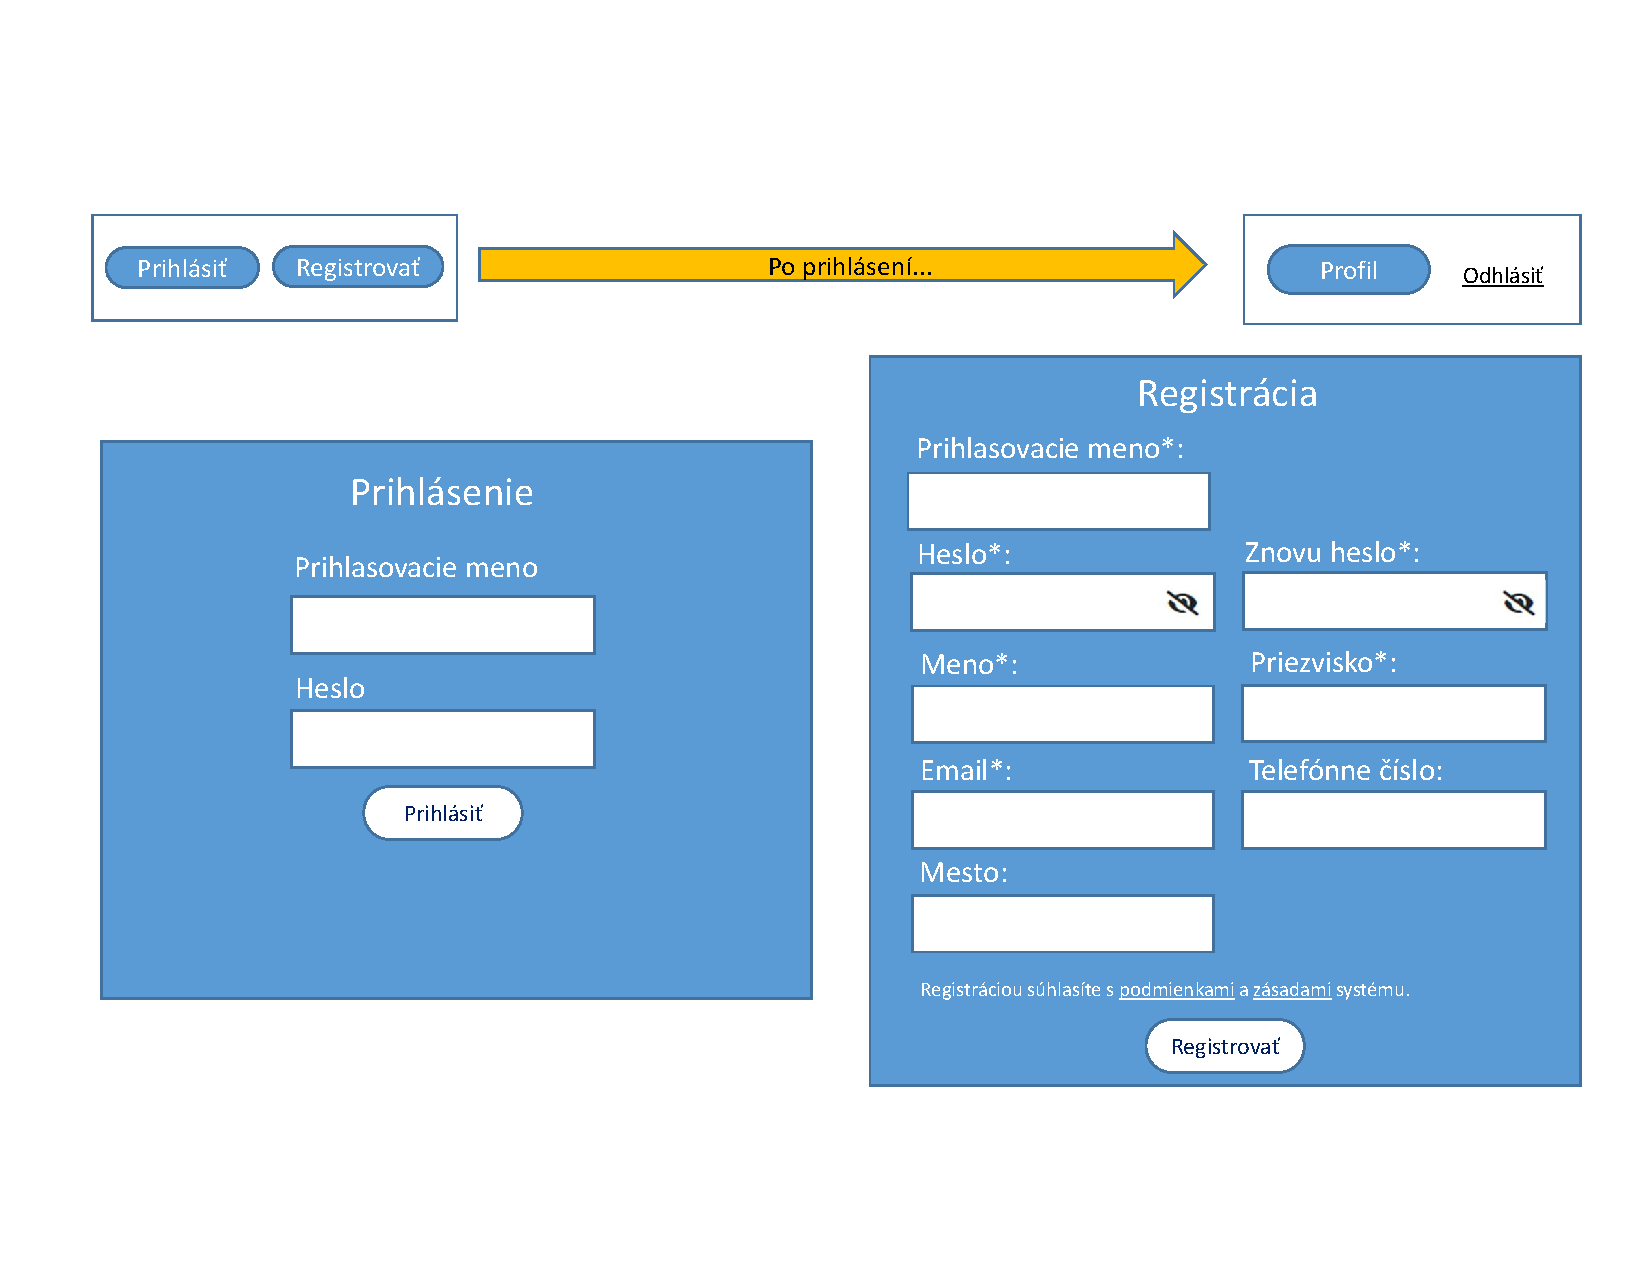
\includegraphics[width=140mm]{../img/UI concept/auth}
\caption{Prihlasovací panel (hore), prihlasovací formulár (vľavo), registračný formulár (vpravo).}
\label{auth}
\end{figure}

Ak je užívateľ prihlásený, tak sa má v~prihlasovacom paneli nachádzať tlačidlo~,,Profil`` a~odkaz ,,Odhlásiť`` (viď~vpravo hore na~obr.~\ref{auth}).

Po~kliknutí na~tlačidlo~,,Profil`` má byť užívateľ presmerovaný do~časti aplikácie s~jeho údajmi.

Po~kliknutí na~odkaz~,,Odhlásiť`` má byť užívateľ odhlásený.

\subsection{Prihlásenie}

TODO

\subsection{Registrácia}

TODO

\subsection{Profil}

Po~kliknutí na~tlačidlo~,,Profil``, ktoré sa má zobrazovať prihláseným užívateľom v~prihlasovacom paneli, má byť užívateľ presmerovaný do~časti aplikácie s~formulárom, ktorý má obsahovať jeho údaje. Užívateľ si bude môcť pomocou tohto formulára svoje údaje upravovať. Navyše nad~formulárom sa má nachádzať nadpis~,,Profil``. Pre~lepšiu predstavu tejto časti aplikácie viď~obr.~\ref{profile}.

\begin{figure}[H]\centering
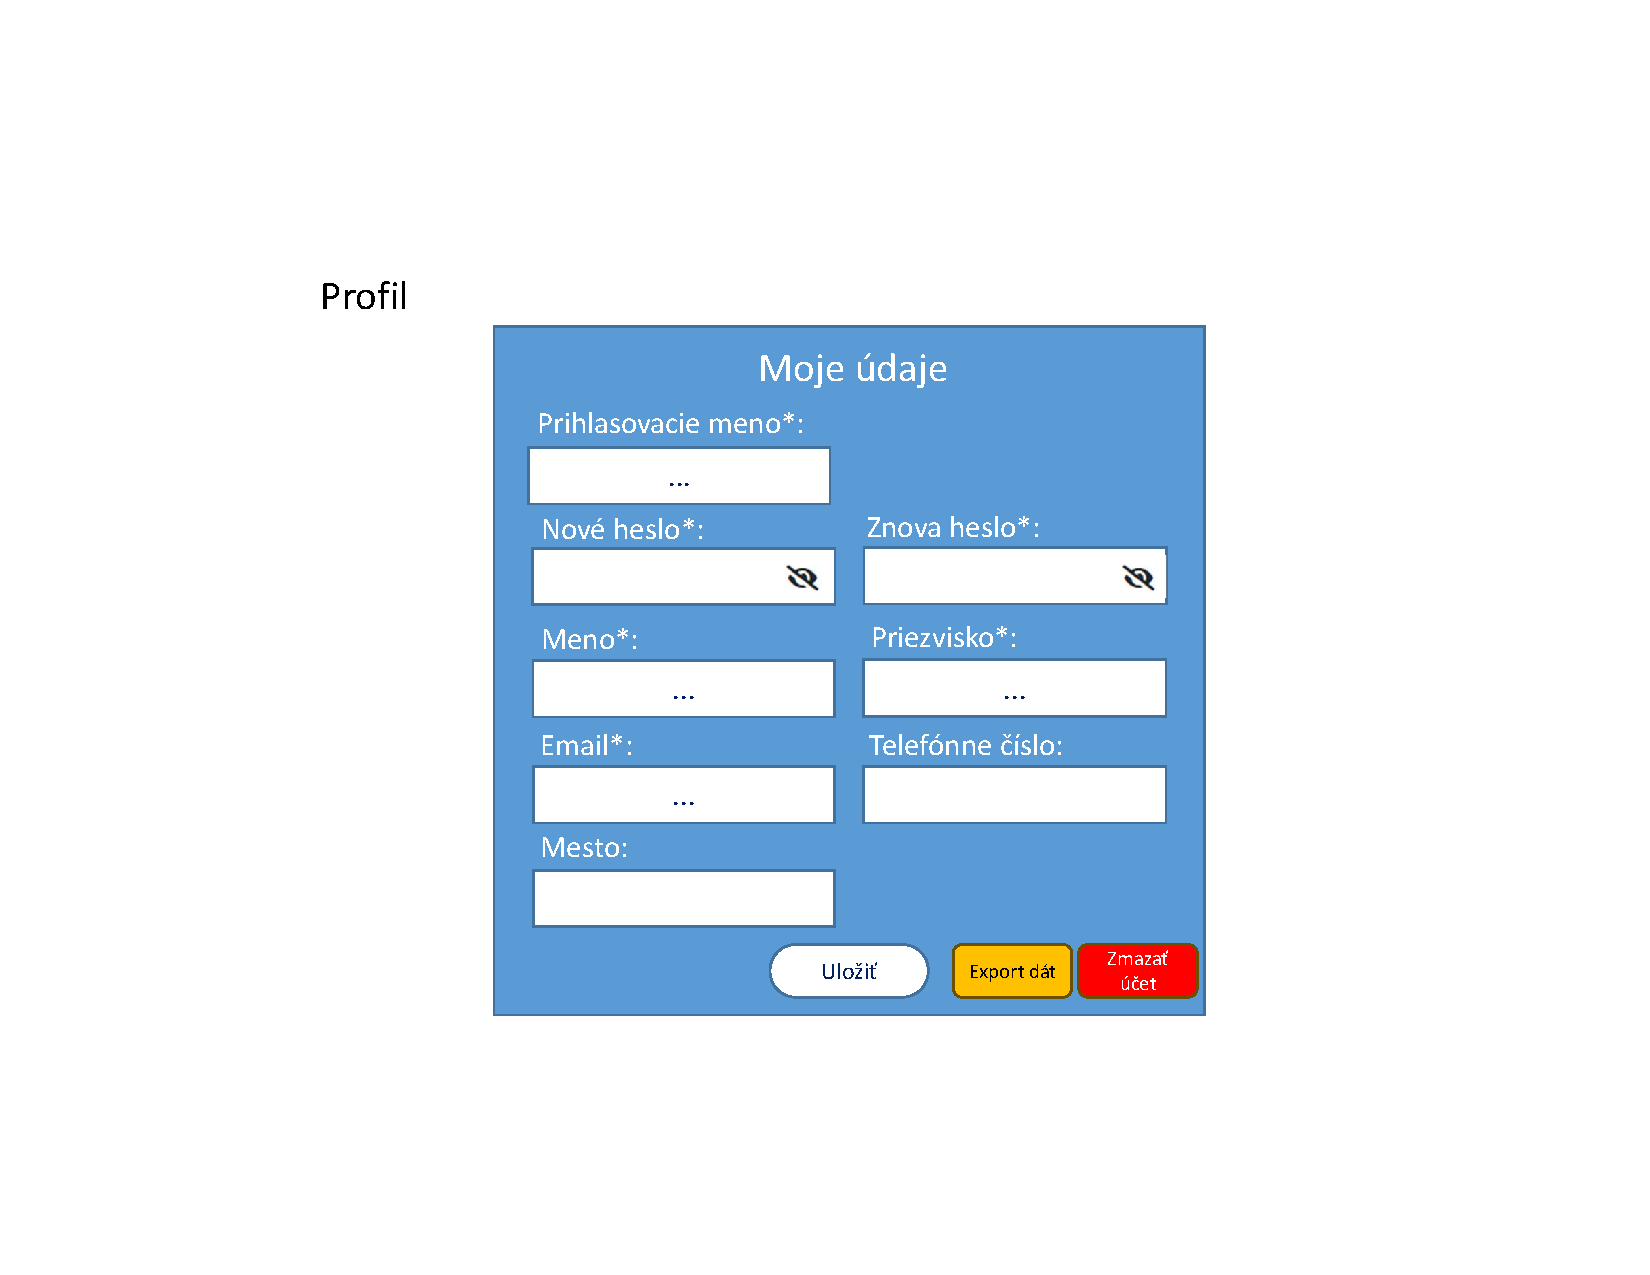
\includegraphics[width=140mm]{../img/UI concept/profile}
\caption{Profil užívateľa}
\label{profile}
\end{figure}

V~hornej časti formulára sa má nachádzať nadpis~,,Moje údaje``. Formulár má obsahovať polia: prihlasovacie meno, heslo, znova heslo, meno, priezvisko, email, telefónne číslo a~mesto. Pričom všetky polia, okrem polí telefónne číslo a~mesto, sú povinné. Povinné polia majú byť označené hviezdičkou.

Všetky polia, až na~polia heslo a~znova heslo, majú byť vyplnené užívateľovými údajmi.

Ak užívateľ začne písať do~poľa heslo alebo~znova heslo, namiesto písmen by sa mali zobrazovať hviezdičky. Pri~týchto poliach by mali byť ikonky, ktoré kliknutím umožnia užívateľovi meniť medzi hviezdičkami a~písmenami v~poliach heslo a~znova heslo. Teda ide o~funkcionalitu zobraziť a~schovať heslo.

Pod~formulárom by sa malo nachádzať tlačidlo~,,Uložiť`` pre~uloženie zmien.

Ak neboli vykonané žiadne zmeny, tak po~kliknutí na~tlačidlo~,,Uložiť`` sa má zobraziť vyskakovacie okno s~textom "Neboli vykonané žiadne zmeny." a~tlačidlom ,,OK``.

Ak užívateľ zinvaliduje nejaké z~polí (napr.~zanechá prázdne povinné pole), má sa zobraziť chybová správa pri~danom poli. Výnimkou sú polia heslo a~znova heslo, tie môžu ostať prázdne. 

Ak by si chcel užívateľ zmeniť heslo, bude musieť vyplniť obe polia, a~ak by obsah polí nebol rovnaký, tak sa má zobraziť vyskakovacie okno s~textom "Obsah políčok \'Nové heslo\' a~\'Znova heslo\' nie sú rovnaké." a~tlačidlom ,,OK``. Alebo ak by si chcel užívateľ zmeniť heslo a~zadal by staré heslo, tak znova sa má zobraziť vyskakovacie okno s~textom "Nové heslo nemôže byť staré heslo." a~tlačidlom ,,OK``.

Po úspešnej zmene údajov sa má zobraziť vyskakovacie okno s~textom "Údaje úspešne zmenené." a~tlačidlom ,,OK``.
